\documentclass[conference]{IEEEtran}
\IEEEoverridecommandlockouts
% The preceding line only needs to identify funding in the first footnote. If that is unneeded, please comment it out.
\usepackage{cite}
\usepackage{amsmath,amssymb,amsfonts}
\usepackage{algorithmic}
\usepackage{graphicx}
\usepackage{textcomp}
\usepackage{xcolor}
\usepackage{subfig}
\usepackage{float}
\usepackage{tabularx}
\usepackage{placeins}
\usepackage{multicol}




\begin{document}

\title{Emergent Behaviours in Heterogeneous Swarms of RVR and BOLT Robots}

\author{\IEEEauthorblockN{Nicholas Liu}
\IEEEauthorblockA{\textit{School of Engineering and Technology} \\
\textit{UNSW Canberra}\\
Canberra, Australia \\
z5364371@ad.unsw.edu.au}}

\maketitle

\begin{abstract}
This project aims to enable the efficient and effective control of a group of autonomous robots through the development and implementation of emergent behaviours within heterogeneous swarms of commercially available RVR and BOLT robots. Emergent behaviours, often observed in the natural world, show significant promise as a decentralised control method of robotic swarms. The swarm's behaviour is governed by a Boid model which utilises local agent behavioural rules of separation, cohesion and alignment to enable a robust and scalable swarm. This project focuses on the tuning of parameters to produce emergent behaviours within a heterogeneous swarm as well as the observation and analysis of those behaviours. This research contributes to the field of swarm robotics by providing a foundational basis for further research into heterogeneous swarms through a low-cost system as well as demonstrating the potential of emergent behaviours for real-world applications such as environmental monitoring and autonomous exploration.     
\end{abstract}

\section{Introduction}

Throughout the natural world, swarms of animals form emergent behaviours, where complex global patterns can be observed across the swarm that originate from local interactions among individual agents. This can be seen in phenomena such as the flocking of birds and schooling of fish, these phenomena show both the possibility for and potential of emergent behaviours. In robotic swarms emergent behaviours have shown significant promise in a computationally efficient and robust method for the organisation and high-level control of a large number of robots \cite{sahin_swarm_2005}.

As the field of swarm robotics has expanded, so has the scope of the problems to be solved by robotic swarms, these include applications in areas such as search and rescue, environmental monitoring and exploration. As the complexity of tasks increases, there is a need for an increasingly complex and versatile swarm. Currently, traditional homogenous swarms, composed of many identical robots with uniform capabilities are limited in their ability to adapt to increasing task complexity. Hence, to expand the capabilities of robotic swarms, heterogeneous swarms have been introduced, which combine different robots within a swarm to increase both capability and adaptability while retaining the characteristics of scalability and robustness that are inherent to robotic swarms \cite{dorigo_swarmanoid_2013}.

The current state of knowledge on emergent behaviours within Boid swarms is primarily focused on homogeneous swarms \cite{jiang_learning_2019,stolfi_optimising_2022}. This narrow view fails to fully capture the potential of emergent behaviours within Boid swarms. By synthesizing together emergent behaviours within a heterogeneous swarm, it is possible to leverage both the robustness and computational efficiency offered through the use of emergent behaviour, along with the enhanced adaptability and capability produced through the use of heterogeneous swarms.

\subsection{Project Aim}

The current knowledge base shows limited applications of heterogeneous swarms on low-cost commercially available robots, furthermore, there is no existing implementation of collective emergent behaviours within heterogeneous swarms in a practical environment, despite emergent behaviours showing a large degree of potential in organising and controlling robotic swarms, promising increased robustness and decreased complexity over traditional formation control techniques. Hence, to address this knowledge gap, the aim of this project is to design and realise a heterogeneous swarm of RVR and BOLT robots, which are widely commercially accessible and available, and to use this swarm to create and observe emergent collective behaviours. This will provide a cost-efficient system that has enhanced capabilities through heterogeneous swarming and will provide a base for further research into the applications of emergent behaviours within heterogeneous swarms.      

\subsection{Project Scope}

The scope of this project includes the development and implementation of emergent behaviours within a physical heterogeneous swarm of robots, in which the primary objective is to bridge the gap in existing research between emergent behaviours in homogeneous swarms and formation control techniques within heterogeneous swarms. 

This project will focus on the practical design and demonstration of emergent behaviours in a robotic swarm comprised of RVR and BOLT robots, this will be achieved through the following key objectives:

\begin{itemize}
    \item \textbf{Heterogeneous Boid Swarm Design and Development}: A system to allow for the heterogeneous swarming of RVR and BOLT robots will be designed with the swarm utilising Reynolds' Boid swarming model \cite{reynolds_flocks_1987}.
    \item \textbf{Emergent Behaviour Parameter Tuning}: To tune the swarming parameters to create emergent behaviour within the heterogeneous swarm, approximate swarming parameters from the literature will be generated and then tuned through observations to create the desired emergent behaviour. 
    \item \textbf{Experimental Analysis and Validation}: Through conducting multiple trials of each emergent behaviour studied and analysing these through the use of swarming metrics, the emergent behaviours produced can be analysed and validated.
\end{itemize}


The scope of this project is confined to the use of the Sphero RVR and BOLT robots as well as the VICON local positioning system, this is to maintain cost efficiency as well as accessibility. This project investigates three hand-tuned emergent behaviours for heterogeneous swarms. These emergent behaviours will become the basis of a machine learning model like reinforcement learning for autonomous tuning of emergent behaviours in heterogeneous swarms in future. Thus this project, aims to build a foundation for future work into heterogeneous swarms through demonstrating the feasibility of realising emergent behaviours in a heterogeneous swarm within a practical environment utilising low-cost platforms.

\section{Relevant Literature}

The field of swarm robotics originated to replicate the unique and efficient swarms observed within the natural world to control a large number of robots \cite{sahin_swarm_2005}, this is realised through the implementation of a large system of agents that interact on a local level through basic rules, this approach allows for large numbers of autonomous robots to be controlled as a scalable, flexible and robust system, making it suitable for highly complex tasks in dynamic environments \cite{brambilla_swarm_2013}. 

In the natural world, swarms develop emergent behaviours to solve distinct and unique problems, Di Marzo Serugendo et al observe how natural behaviours are replicated within swarm robotics to solve similar problems \cite{di_marzo_serugendo_self-organisation_2004}, while van Diggelen et al analyse how specialised collective behaviours emerge within heterogeneous swarms of ants and how to implement this computationally \cite{van_diggelen_emergence_2024}. These papers show the importance of designing robotic swarms capable of emergent behaviours, as these prove to be incredibly simple, providing significant scalability and robustness into the swarm as well as specialising and optimising the swarm for certain tasks. 

\subsection{Swarming Models and Algorithms}

To model the swarms observed within nature, the field of swarm robotics has developed various swarming algorithms that enable multi-agent systems to coordinate themselves to complete complex tasks. In 1986, Craig Reynolds conceptualised the first computational swarming algorithm to model the flocking of birds \cite{reynolds_flocks_1987}, this was through the implementation of three rules each agent followed, separation, to avoid collisions with nearby agents, alignment, to move in the average heading of nearby agents and cohesion, to move toward the average position of nearby agents. This swarming model proved to be foundational in developing an understanding of swarm robotics. 

As swarm robotics has developed new algorithms have been implemented to control robotic swarms, most significantly particle swarm optimisation developed in 1995 by Kennedy et al \cite{kennedy_particle_1995} controls robotic swarms through an iterative optimisation method with agents attempting to find the optimal solution to a problem. Furthermore, Dorigo et al \cite{dorigo_ant_1999} developed an ant-inspired pheromone-based swarming model which proved useful in path planning and routing. As research into swarm robotics continued further mimicry of natural phenomena was developed, Karaboga et al \cite{karaboga_idea_2005} in 1995 conceptualised an artificial bee colony algorithm to model bees searching for pollen in a meta-heuristic approach to optimise problems, in 2009, Yang et al \cite{yang_firefly_2009} developed the firefly algorithm, inspired by the flashing of fireflies, thus these show how natural behaviours can be reflected through meta-heuristic algorithms to form models of large swarms.

Each of these algorithms offers different advantages and disadvantages, for this project the Reynolds Boids model was used over an optimisation type model as the Boids model created a swarm that did not seek to reach a goal state, thus being an ideal environment in which to produce emergent behaviours. This has been previously done in a homogeneous environment by Abpeikar et al. \cite{abpeikar_iterative_2023} utilising the Boid swarming model, to extend on this this project seeks to implement emergent behaviours on a heterogeneous swarm. 

\subsection{Emergent Behaviours in Swarm Robotics}

Emergent behaviours can be observed within the natural world, such as birds flocking and ants moving in a line, these are complex global patterns that arise from local interactions between individuals within a swarm \cite{di_marzo_serugendo_self-organisation_2004}, and these are most likely evolved through the process of natural selection. In robotic swarms emergent behaviours allow agents to efficiently organise and optimise themselves as individuals for a given task, this provides an increased adaptability and robustness to the use of emergent behaviours over traditional swarming and formation control methods. 

Current research into emergent behaviours within robotic swarms is primarily focused on the use of homogeneous swarms, for instance, Hamann applies a model to predict the future of the system and produced emergent behaviours in simulation \cite{hamann_evolution_2014}, this produced behaviours such as dispersion, aggregation and flocking. The Reynolds Boids model is ideal for the study and production of emergent behaviours as it produces a swarm that does not have a goal in mind, this is evident throughout existing literature, for instance, Khan et al produced a fitness function to analyse Boid swarms for behaviours of interest and to subsequently generate emergent behaviours \cite{khan_autonomous_2020}, furthermore, Abpeikar et al \cite{abpeikar_iterative_2023} applied simulation pre-trained behaviours through transfer learning to a material swarm of Sphero BOLT robots.

However, within the current literature, there is no practical implementation of emergent behaviours within a heterogeneous swarm, this project aims to address this gap and to create a heterogeneous swarm that benefits from the increased adaptability and robustness of emergent behaviours. 

\subsection{Heterogeneous Swarms}

A heterogeneous swarm consists of multiple different species of robot, each with differing capabilities and functionality, this results in a swarm with enhanced adaptability and flexibility through leveraging the diversity of the swarm through the optimisation and specialisation of each species of robot \cite{dorigo_swarmanoid_2013}. While current research focuses on the use of homogeneous swarms, heterogeneous swarms can solve problems of greater complexity in more dynamic environments by leveraging the potential found within the diversity of agents. Heterogeneity within swarms can be defined as either physical or behavioural, through physical heterogeneity; agents can be equipped with varying hardware required for species-specific tasks, and behavioural heterogeneity; species are specialised and optimised for different tasks \cite{dorigo_reflections_2020}.

While research is currently dominated by homogeneous swarms \cite{brambilla_swarm_2013}, heterogeneous swarms have begun to gain traction, in 2013 Dorigo et al developed and implemented the Swarmanoid heterogeneous swarm consisting of eye, hand and foot bots \cite{dorigo_swarmanoid_2013}, this represented the first realised heterogeneous robotic swarm with each species within the swarm having unique capabilities. This swarm demonstrated the potential of a heterogeneous swarm in the execution of complex tasks in dynamic environments. Other novel approaches to heterogeneous swarming include a "shepherding" technique where larger and more complex robots command and control groups of smaller more agile robots \cite{pinciroli_coordinating_2010}. Prorok et al utilised a decentralised optimisation method to coordinate heterogeneous swarms between multiple species-specific tasks, highlighting the enhanced ability of heterogeneous swarms to address multiple problem types simultaneously \cite{prorok_impact_2017}. Other swarm and formation control methods include a particle swarm optimisation-based application by Inácio et al \cite{inacio_pso-based_2019}, as well as a Boid model implemented in a heterogeneous swarm simulation by Momen et al \cite{momen_mixed_2007}. While the current literature explores Boid models in heterogeneous swarms, there is a notable absence of practical implementations in real-world environments.

This project aims to address this gap through the design and development of a heterogeneous Boid swarm in a real-world environment utilising low-cost platforms that produce emergent behaviours, demonstrating the synthesis of the scalable and robust nature of emergent behaviours with the versatile and flexible nature of heterogeneous swarms. This will form the foundation for further research into the applications of emergent behaviours in heterogeneous Boid swarms. 

\section{Heterogeneous Swarm Design Methodology}

The approach for this project first worked to develop the heterogeneous swarming system, which is defined by the ability to operate a multi-agent system comprised of Sphero RVR and BOLT robots, this was approached through two different methods, a decentralised and centralised swarm control approach.  

To develop and tune the parameters required for each emergent behaviour the speed and heading of agent class (RVR and BOLT) were first normalised, following this the process for tuning for a specific emergent behaviour was through experimentation; by using pre-existing homogeneous Boid parameters implemented on Sphero BOLTs developed by Abpeikar et al \cite{abpeikar_mechanism_2023}, as well as through linearly scaling parameters determined through simulation by Khan et al \cite{khan_autonomous_2020} and adjusting these parameters intuitively. 

\subsection{Robot Setup and Local Positioning System}

Within this project three distinct subsystems were used: the Sphero BOLT robot, Sphero RVR robot and VICON local positioning system. The BOLT is a spherical robot depicted in figure \ref{fig:bolt}, housing an onboard microcontroller to receive commands from Bluetooth low energy and execute commands. It further maintains its own position, heading and velocity through an onboard IMU and magnetometer. 

While the Sphero RVR depicted in figure \ref{fig:rvr} has similar capabilities to the Sphero BOLT, it is a tank-drive style robot. It additionally sends and receives data over UART to an attached Raspberry Pi 3B+, providing the RVR with both WiFi and Bluetooth communication capabilities. 

The VICON system consists of eight cameras that utilise retro-reflective markers to detect the location of robots in the experiment area, sending data over LAN. The BOLT and RVR robot setups are depicted in Figures \ref{fig:bolt}, \ref{fig:rvr}, the BOLT utilises a cup with VICON markers to allow for the ball to rotate underneath while still maintaining connectivity.

\begin{figure} [h]
    \centering
    \parbox{3.5cm}{
    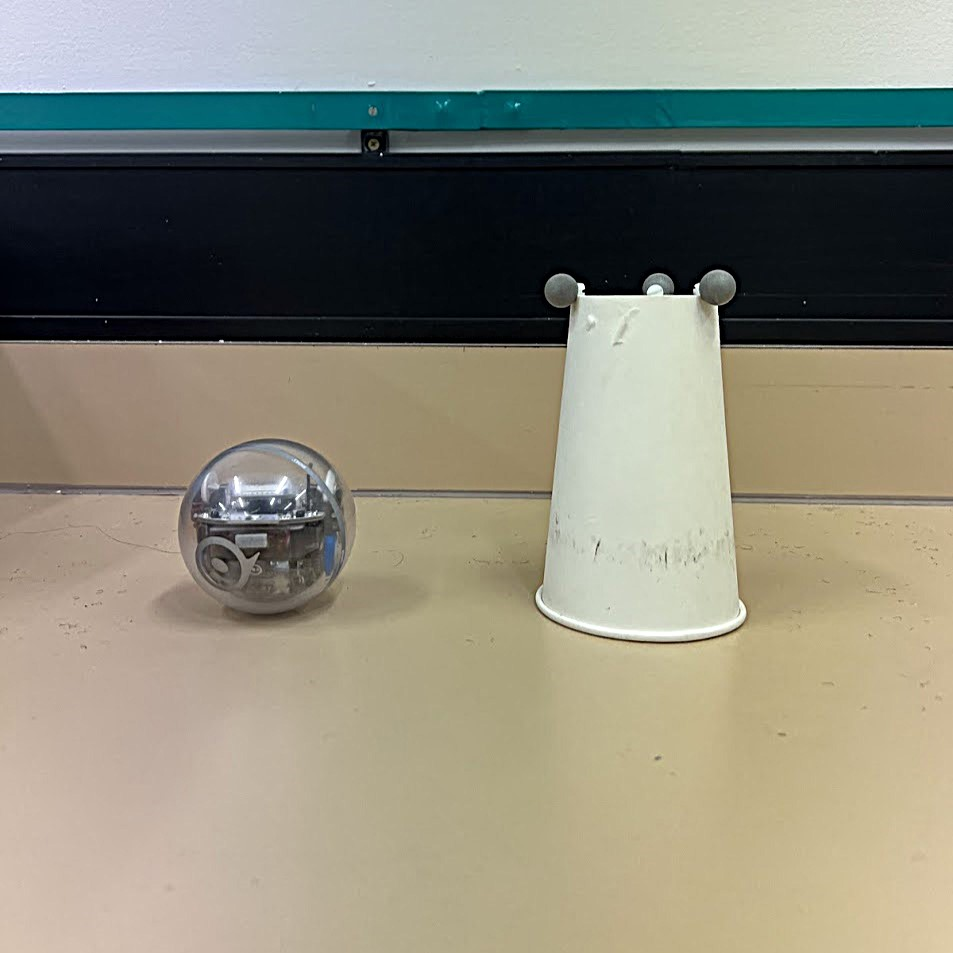
\includegraphics[width=3.5cm]{BOLT image.jpg}
    \caption{BOLT Setup}
    \label{fig:bolt}}
    \qquad
    \begin{minipage}{3.5cm}
    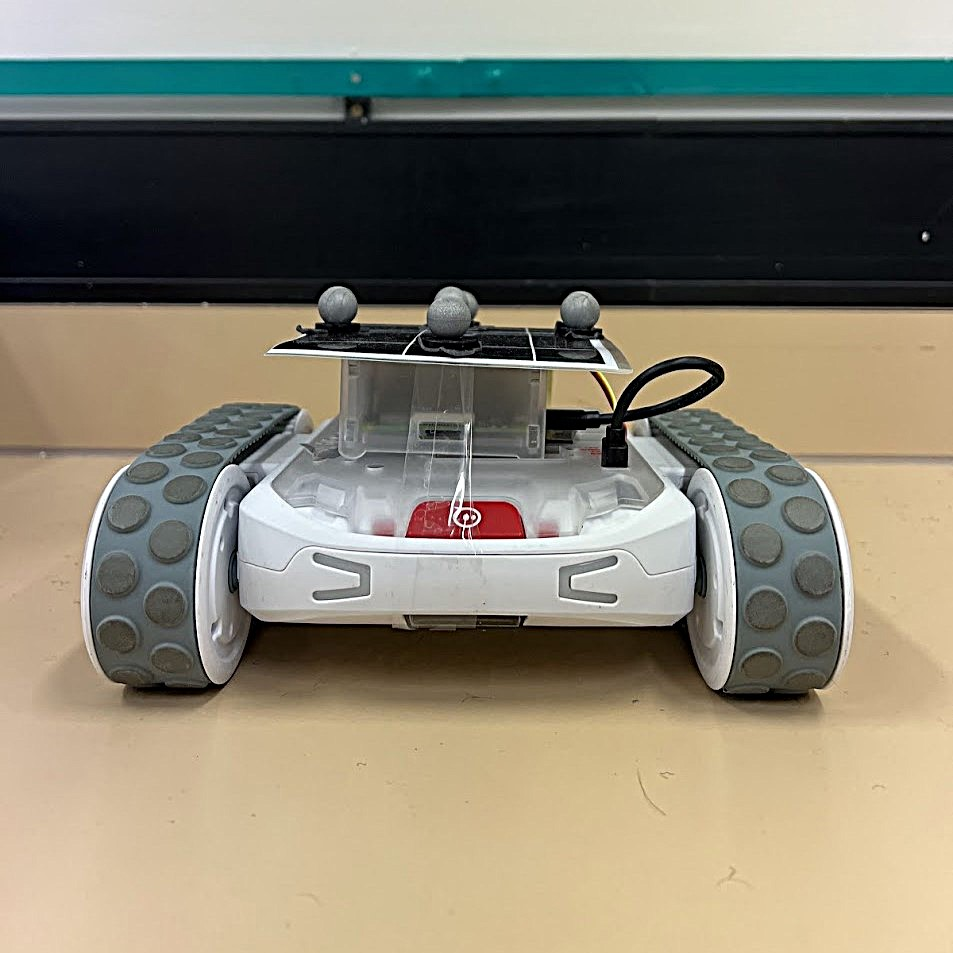
\includegraphics[width=3.5cm]{RVR Image.jpg}
    \caption{RVR Setup}
    \label{fig:rvr}
    \end{minipage}
\end{figure}

\FloatBarrier

\subsection{Implementation of Boid Algorithm}
Each agent individually calculates its own updated velocity based on its neighbouring agents through the use of the rules of cohesion, alignment and separation \cite{reynolds_flocks_1987}. Within the heterogeneous swarming system, each Boid object requests the central Swarm object for the centre of mass and average heading of all neighbours within its vision range and angle. In the Boid algorithm, each agent $A^i$ considers its neighbouring agents $N^i$ defined as:
\begin{equation}
N^i = \left\{ A^k \ne A^i\ \land\ \text{dist}(A^k, A^i) < R \right\}
\label{eq1}
\end{equation}
Where $\text{dist}(A^k, A^i)$ represents the Euclidean distance between agents $A^k$ and $A^i$, and $R$ is the interaction radius.

The individual force derived from each rule is then calculated through the use of the parameters of radius and weight:

For cohesion, agent $A^i$ calculates the average position $\bar{c}_t^i$ of neighboring agents $A^k$ within range $R_c$:
\begin{equation}
\bar{c}_t^i = \frac{\sum_k x_t^k}{\left| (N_{c})_t^i \right|}
\label{eq2}
\end{equation}
Where $x_t^k$ is the position of agent $A^k$ at time $t$, and $\left| (N_{c})_t^i \right|$ is the number of neighbours within the cohesion radius $R_c$ at time $t$.

The cohesion vector $c_t^i$ is then calculated as the vector from agent $A^i$ towards $\bar{c}_t^i$:
\begin{equation}
c_t^i = \bar{c}_t^i - x_t^i
\label{eq3}
\end{equation}

Similarly, for separation, the agent calculates the average position $\bar{s}_t^i$ of neighbours within the separation radius $R_s$:
\begin{equation}
\bar{s}_t^i = \frac{\sum_k x_t^k}{\left| (N_{s})_t^i \right|}
\label{eq4}
\end{equation}
The separation vector $s_t^i$ is calculated as the vector away from $\bar{s}_t^i$:
\begin{equation}
s_t^i = x_t^i - \bar{s}_t^i
\label{eq5}
\end{equation}

For alignment, the agent calculates the average velocity $\bar{a}_t^i$ of neighbors within the alignment radius $R_a$:
\begin{equation}
\bar{a}_t^i = \frac{\sum_k v_t^k}{\left| (N_{a})_t^i \right|}
\label{eq6}
\end{equation}

These vectors are subsequently combined at each timestep to update the velocity and heading of agent $A^i$:
\begin{equation}
v_{t+1}^i = v_t^i + W_c c_t^i + W_a a_t^i + W_s s_t^i
\label{eq7}
\end{equation}

\subsection{Development of Heterogeneous Swarming System}

The development of the heterogeneous swarming system presented multiple challenges involving several critical milestones. These were primarily caused by the differing access levels available to each agent control system. The RVR utilised a fully integrated and unlocked control system through the sphero-sdk library provided by the manufacturer, while the BOLT uses an unofficial library, spherov2 to interface with the BOLT over bleak, a python Bluetooth low energy adapter.

The first milestone was to develop a communication system across all classes of agents. The difficulty here arose due to the different nature of the RVR and BOLT robot's communications protocols, with RVR robots using WiFi with a poorly implemented Bluetooth transceiver, while the BOLT robots only functioned through Bluetooth. This problem was compounded by the differing APIs used to control each class. This promoted the second milestone: developing both the individual agent control system as well as the multi-agent framework which required multiple different instances to be hosted on one central swarm controller. 

The first approach to producing a heterogeneous swarming system was to produce a \textbf{decentralised} system that lacked a central swarm controller and allowed each RVR and BOLT to operate as independent agents. This was attempted due to the benefit of a realised decentralised heterogeneous robotic swarm, which would take on many aspects of a decentralised heterogeneous multi-agent system, such as one developed by Hudson et al for subterranean exploration \cite{hudson_heterogeneous_2022} while maintaining the scalability and robustness of swarming systems.

The second approach to the problem was to implement a \textbf{centralised} swarm controller to control all swarming agents. This allowed a faster and less complex communications scheme to be implemented. By using a central swarm controller coupled with agent-specific APIs and classes each agent could be controlled as if the swarm was computationally homogeneous.

\subsection{Swarm Communications Schematic} 

The heterogeneous swarming system required three distinct elements to communicate with each other between the BOLT, RVR and VICON systems. The BOLT and RVR agents had to have the capability to send and recover their respective speech and headings while the swarm controller needed to interface with the VICON system to update the locations of each robot. 
While both BOLT and RVR are capable of infrared communications, the APIs available have a limited implementation of this and therefore it was not possible to implement this type of communication. During initial development, a decentralised communication scheme was designed and tested as seen in Figure \ref{fig:Old Schema}, this faced multiple challenges including:
\begin{itemize}
    \item The Raspberry Pi was unable to maintain a reasonable execution speed for multiple threads, due to simultaneously managing data from VICON and controlling the RVR and multiple BOLT robots simultaneously, resulting in agents not updating velocity within a reasonable time frame.
    \item The Bluetooth connectivity between BOLT robots and the RVR robot's onboard Raspberry Pi was unstable and prone to instability 
\end{itemize}
Thus for these reasons above the decentralised system was rebuilt with a centralised swarm controller in mind to alleviate these issues. 

\begin{figure}[htbp]
    \centering
    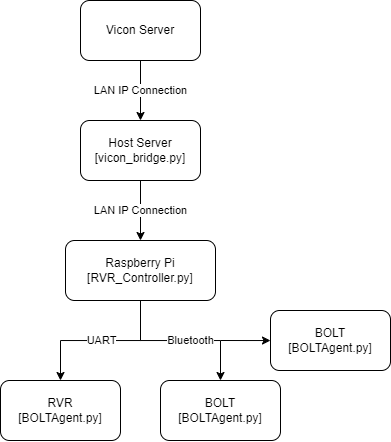
\includegraphics[width=0.75\linewidth]{first communication Scheme.drawio (1).png}
    \caption{De-Centralised Communication Scheme}
    \label{fig:Old Schema}
\end{figure}

 Shown in Figure \ref{fig:New Schema} is the implemented centralised communication schema showing the use of the Python bleak library to interface with BOLTs and network sockets to pass instructions to RVRs and LAN connection to pull data from the VICON positioning system. This approach used a significantly stronger and hence more stable Bluetooth adaptor through the centralised swarm controller, furthermore, this reduced the number of calculations required per time-step for each thread, as it no longer required VICON data to be streamed or for RVRs to broadcast location data over LAN, resulting in faster velocity updates and hence smoother swarming. Thus, the solution to the communication milestone was to implement a centralised control system that sends and receives data from each agent. 

\begin{figure}[htbp]
    \centering
    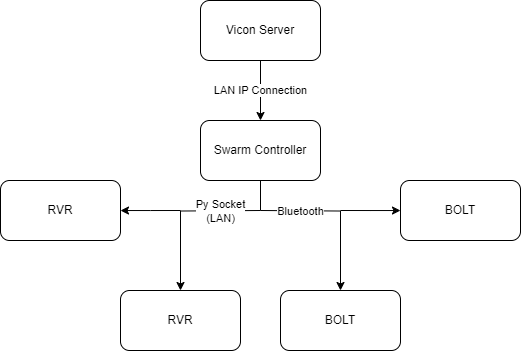
\includegraphics[width=1\linewidth]{new system.drawio.png}
    \caption{Centralised Communication Scheme}
    \label{fig:New Schema}
\end{figure}

\subsection{Swarm Agent Framework}

The second key milestone overcome was the development of a multi-agent framework that performed Boid-swarming calculations for each agent and executed their reactions to their respective observed environments continuously and simultaneously. This was achieved through each agent being declared as its own object with individual attributes such as position, speed and heading, this was used with a larger overall object that stored the locations of each element of the swarm and thus could execute requests for the swarm alignment and centre of mass from the point of view of any agent with a respective radius and field of view. Then through threading the swarm controller operated multiple different agent objects simultaneously to successfully execute a heterogeneous swarm, this layout is depicted in Figure \ref{fig:New Schema}. A breakdown of each element is provided below: 

\begin{itemize}

    \item \textbf{VICON Locator}: this class runs in the background to maintain a LAN connection to the VICON system through the VICON DataStreaming SDK, it ensures that location data can be pulled on demand.
    
    \item \textbf{Boid BOLT}: this class is used for each BOLT agent, it receives its position from the VICON Locator class mentioned above and its speed and heading from the BOLT interface. It calculates a new speed and heading based on Boid forces and pushes these across Bluetooth using the BOLT interface.
    
    \item \textbf{Boid RVR}: this class is used for each RVR agent, it receives its position from the VICON Locator class mentioned above and its speed and heading are taken from the last speed and heading passed to the robot. Onboard the RVR, the Raspberry Pi receives an updated speed and heading from the Boid RVR class through a network socket and passes it to the RVR through UART.
    
    \item \textbf{Swarm Controller}: this class hosts all swarming agents and performs the calculation of the Boid forces of separation cohesion and alignment, this is achieved through the class pulling the positions, speeds and headings of each agent within the swarm and can hence determine the swarm average heading and centroid based on the radius and field of vision provided.  
    
\end{itemize}


\section{Experimental Methodology}

\subsection{Environmental Setup}

To form emergent behaviour within the heterogeneous swarm two BOLT and two RVR robots would be used, with an experimental setup of two BOLTs behind two RVR robots initially, each experiment would be run with a set of swarming parameters which varied between the BOLT and RVR due to speed scaling differences, all agents were bound within an imaginary two by two metre box, this setup can be seen in figure \ref{fig:experiment setup}.

\begin{figure} [h]
    \centering
    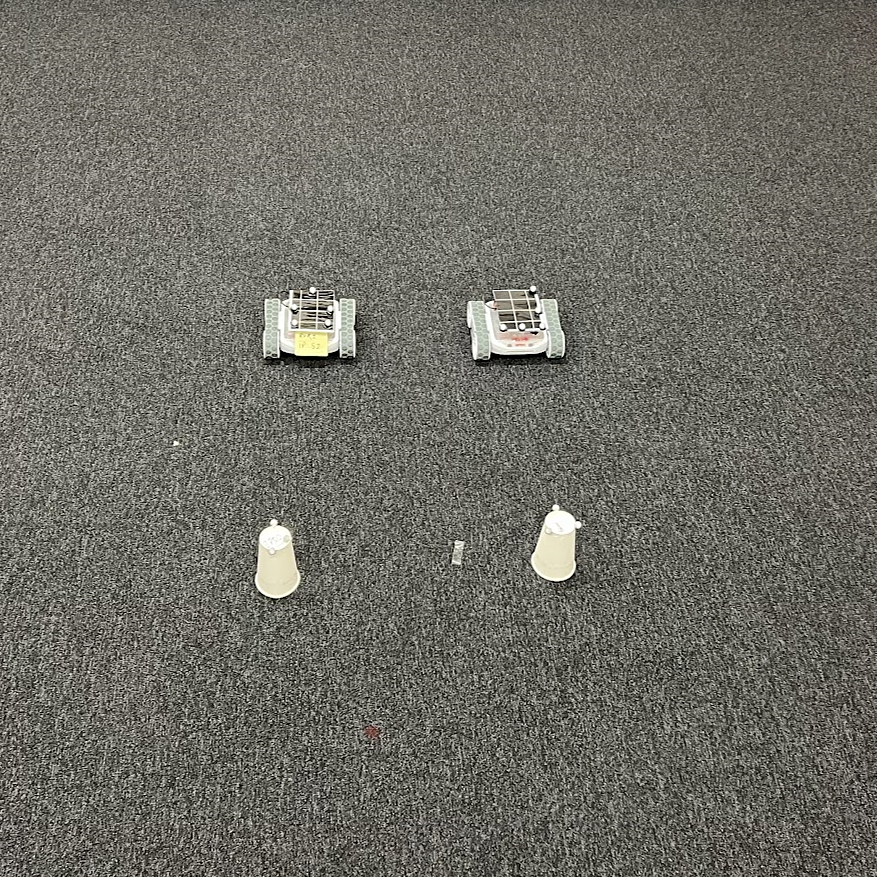
\includegraphics[width=0.55\linewidth]{Experimental Setup.png}
    \caption{Initial Positions of Robots}
    \label{fig:experiment setup}
\end{figure}

For data collection, four trials were run for each behaviour with the use of the VICON recording system to log data and accurately determine the position, speed and heading of each robot, this external data logging method was conducted in order to mitigate the issue of sensor drift within the robot's internal systems as well as to reduce computational load on the swarm controller, as these caused erratic behaviour throughout initial testing.

\subsection{Validation and Experimental Studies}

To analyse each swarming behaviour both locations across time were plotted as well as swarming metrics were calculated, these are derived from the paper by Yang et al \cite{yang_automatic_2023}, and these characterise each swarm and show the difference between random motion and swarming. To both verify the swarming system as well as to understand the impact of each Boid parameter of separation cohesion and alignment, a series of parameter studies were conducted:

\begin{itemize}

\item \textbf{BOLT Swarm}: This study utilised three BOLT robots to conduct a homogeneous swarming study to verify the swarming system

\item \textbf{RVR Swarm}: Similar to the BOLT study, this study utilised three RVR robots in a homogeneous configuration

\item \textbf{Heterogeneous Test}: This was the initial test conducted with two BOLT robots and one RVR robot to confirm the functionality of the swarm controller in a heterogeneous format

\item \textbf{Flocking Study}: This study was run with two BOLT and two RVR robots, it was conducted by initially beginning with the flocking parameters from the paper by Abpeikar et al \cite{abpeikar_iterative_2023} that was successfully used with BOLTs, this was performed multiple times in different configurations to tune the swarming parameters to produce the end result.

\item \textbf{Line Study}: Similarly to the study above, this study initially began with line following parameters from the paper by Khan et al \cite{khan_autonomous_2020} that was successfully used with BOLTs, this was performed multiple times in different configurations to tune the parameters to produce the end result.

\item \textbf{Gravity Study}: This study was conducted with two BOLT and two RVR robots to produce a gravity-type swarm formation, characterised by swarms orbiting an imaginary central point, the initial parameters utilised from the literature were first produced by Khan et al \cite{khan_autonomous_2020}.

\item \textbf{Random Study}: This study was achieved by using two BOLT and two RVR robots and having set all weights to null, resulting in no swarming.

\end{itemize}

\subsection{Parameter Tuning}
Within Boid swarms, under the correct conditions set through the swarming parameters, it is possible for the swarm to form emergent behaviours such as flocking and line following \cite{kasmarik_autonomous_2020}, through the study and analysis of the parameters derived from simulations by Kasmarik et al \cite{kasmarik_autonomous_2020} and those implemented on Sphero BOLTs by Abpeikar et al \cite{abpeikar_automatic_2022}, a method of implementing and adjusting the parameters used successfully within the paper by Abpeikar et al \cite{abpeikar_automatic_2022} was devised.  

The four targeted behaviours selected for this project represent different types of functional emergent behaviour, these are flocking, line following, a novel swarming behaviour to understand the interactions between the two agent classes as well as a control behaviour of random motion with no swarming. Each of these emergent behaviours has real-world benefits and applications outside of the experimental environment, due to their optimised motion and layout for certain tasks. 

The initial parameters for each emergent behaviour were determined through the examination of previous literature and experimentation undertaken by Khan et al, who produced emergent behaviours in simulation through the use of a machine learning model, and Abpeikar et al, who implemented these behaviours within a homogeneous swarm of Sphero BOLT robots \cite{khan_autonomous_2020,abpeikar_iterative_2023}, these were modified over a regimen of trial and error, with the both independent and simultaneous tuning of parameters. Parameter adjustments (hand-tuned parameters) were made through observation, if robots formed species-independent subgroups the parameters were independently adjusted, otherwise, the parameters were simultaneously adjusted to create emergent behaviours. The metrics of each run during initial parameter tuning can be observed in Appendix A, initial parameters are shown in table \ref{tab0}.

\begin{table}[h]
\centering
\caption{Initial Parameters for Emergent Behaviour Studies}
\label{tab0}
\begin{tabular}{|c|c|c|c|c|c|c|}
\hline
\textbf{Parameter}     & \multicolumn{2}{|c|}{\textbf{Flocking}} & \multicolumn{2}{|c|}{\textbf{Line}} & \multicolumn{2}{|c|}{\textbf{Gravity}} \\  \hline
\textbf{Agent Type}    & BOLT               & RVR              & BOLT             & RVR            & BOLT              & RVR              \\ \hline
$\mathbf{R_c}$         & 100                & 100              & 100              & 100            & 400               & 400              \\ \hline
$\mathbf{R_a}$         & 50                & 50               & 100              & 100            & 400               & 400              \\ \hline
$\mathbf{R_s}$         & 25                 & 35               & 25               & 25             & 25                & 25               \\ \hline
$\mathbf{W_c}$         & 0.3                & 1.0              & 1.0              & 1.0            & 1.0               & 1.0              \\ \hline
$\mathbf{W_a}$         & 0.8                & 1.5              & 1.0              & 1.3            & 0                 & 0                \\ \hline
$\mathbf{W_s}$         & 0.1                & 1.2              & 0                & 0              & 0.44              & 0.44             \\ \hline
$\mathbf{\theta_{vision}}$ & 360            & 360              & 180              & 180            & 360               & 360              \\ \hline
$\mathbf{V_{min}}$     & 50                 & 80               & 50               & 75             & 50                & 75               \\ \hline
$\mathbf{V_{max}}$     & 70                & 100              & 75               & 105            & 75                & 105 \\ \hline             
\end{tabular}
\end{table}

Initially, tuning was tedious due to the requirement to test and understand the effects of different Boid parameters across different species of robot, this was compounded by both sensor drift within robots as well as poor Bluetooth connectivity. The experimental approach towards parameter tuning was to utilise the parameters from literature and to adapt them for a heterogeneous swarm by normalising the radii and weights as well as scaling velocities between both species. The tuned parameters for each behaviour are depicted within table \ref{tab1}


\begin{table}[h]
\centering
\caption{Parameters Tuned for Emergent Behaviour Studies}
\label{tab1}
\begin{tabular}{|c|c|c|c|c|c|c|}
\hline
\textbf{Parameter}     & \multicolumn{2}{|c|}{\textbf{Flocking}} & \multicolumn{2}{|c|}{\textbf{Line}} & \multicolumn{2}{|c|}{\textbf{Gravity}} \\  \hline
\textbf{Agent Type}    & BOLT               & RVR              & BOLT             & RVR            & BOLT              & RVR              \\ \hline
$\mathbf{R_c}$         & 100                & 100              & 100              & 100            & 400               & 400              \\ \hline
$\mathbf{R_a}$         & 75                 & 50               & 100              & 125            & 400               & 400              \\ \hline
$\mathbf{R_s}$         & 50                 & 35               & 25               & 25             & 25                & 25               \\ \hline
$\mathbf{W_c}$         & 1.0                & 1.0              & 1.0              & 1.0            & 1.0               & 1.0              \\ \hline
$\mathbf{W_a}$         & 1.3                & 1.5              & 1.0              & 1.3            & 0                 & 0                \\ \hline
$\mathbf{W_s}$         & 1.2                & 1.2              & 0                & 0              & 0.44              & 0.44             \\ \hline
$\mathbf{\theta_{vision}}$ & 360            & 360              & 180              & 180            & 360               & 360              \\ \hline
$\mathbf{V_{min}}$     & 50                 & 75               & 50               & 75             & 50                & 75               \\ \hline
$\mathbf{V_{max}}$     & 75                 & 105              & 75               & 105            & 75                & 105 \\ \hline             
\end{tabular}
\end{table}

\FloatBarrier
\section{Results and Discussion}

The swarming metrics calculated derived from Yang et al \cite{yang_automatic_2023} are the grouping, order and subgroup counts, each of these provide key insight into each part of the swarm. Grouping is a measure of cohesion; how connected a swarm is and represents the average separation distance between Boids. Greater groupings with less stability represent inconsistent and spread out swarms, while lesser groupings with higher stability represent consistent, closer swarms, it is calculated through:

\begin{equation}
s_i = \frac{1}{n - 1} \sum_{j=1}^{n} \|b_i, b_j\|
\label{eq:grouping}
\end{equation}

\noindent \textbf{Where:}
\begin{IEEEeqnarray} {rCl}
    s_i & : & \text{Average distance for agent } i \\
    n   & : & \text{Total number of agents in swarm} \\
    b_i & : & \text{The } i\text{-th agent in swarm} \\
    b_j & : & \text{The } j\text{-th agent in swarm, for } j = 1, 2 \dots n 
    \end{IEEEeqnarray}

Order represents the alignment of the velocities of a swarm, a lower order represents swarms with increased deviations and inconsistencies while a higher order represents almost perfect movement and is calculated through:

\begin{equation}
Order = \frac{1}{n}|\sum_{i=1}^{n} v_i|
\label{eq:order}
\end{equation}

\noindent \textbf{Where:}
\begin{IEEEeqnarray} {rCl}
    n   & : & \text{Total number of agents in swarm} \\
    v_i & : & \text{The velocity of } i\text{-th agent in swarm} 
\end{IEEEeqnarray}

Subgroup count is calculated through the use of Density-Based Spatial Clustering of Applications with Noise (DBSCAN) \cite{ester_density-based_1996}, which is a spatial clustering method. By clustering and grouping the locations of the swarm subgroups can be identified and counted, this count represents the cohesiveness of a swarm and its tendency to either stay together or to deviate and separate from itself and form other swarms. For this purpose $\epsilon$ - neighbourhood was set to fifty centimetres, as well as the minimum count being two, this allowed for the identification of both separate swarms forming as well as agents failing to format swarm.

For each emergent behaviour, four trials were run and locations were recorded through the VICON local positioning, from each trial three thousand VICON frames were taken to calculate the swarming metrics, these were then plotted on each run as seen in Appendix B, below the plots show all runs plotted together with a 95\% confidence interval given for the average grouping, order and subgroup count achieved across each trial. 
\subsection{Random Motion}
    \begin{figure}[htbp]
        \centering
        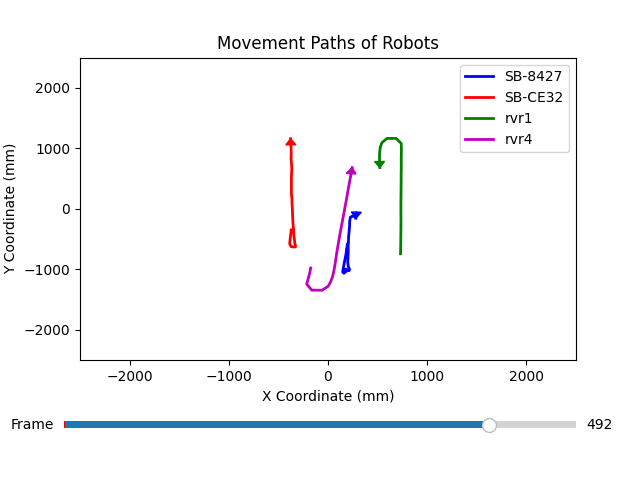
\includegraphics[width=0.45\textwidth]{location_plots/Brownian.png}
        \caption{Random Behaviour Movement Paths, each colour corresponds to a separate agent within the swarm}
        \label{fig:brownian_plot}
    \end{figure}
    \begin{figure}[htbp]
        \centering
        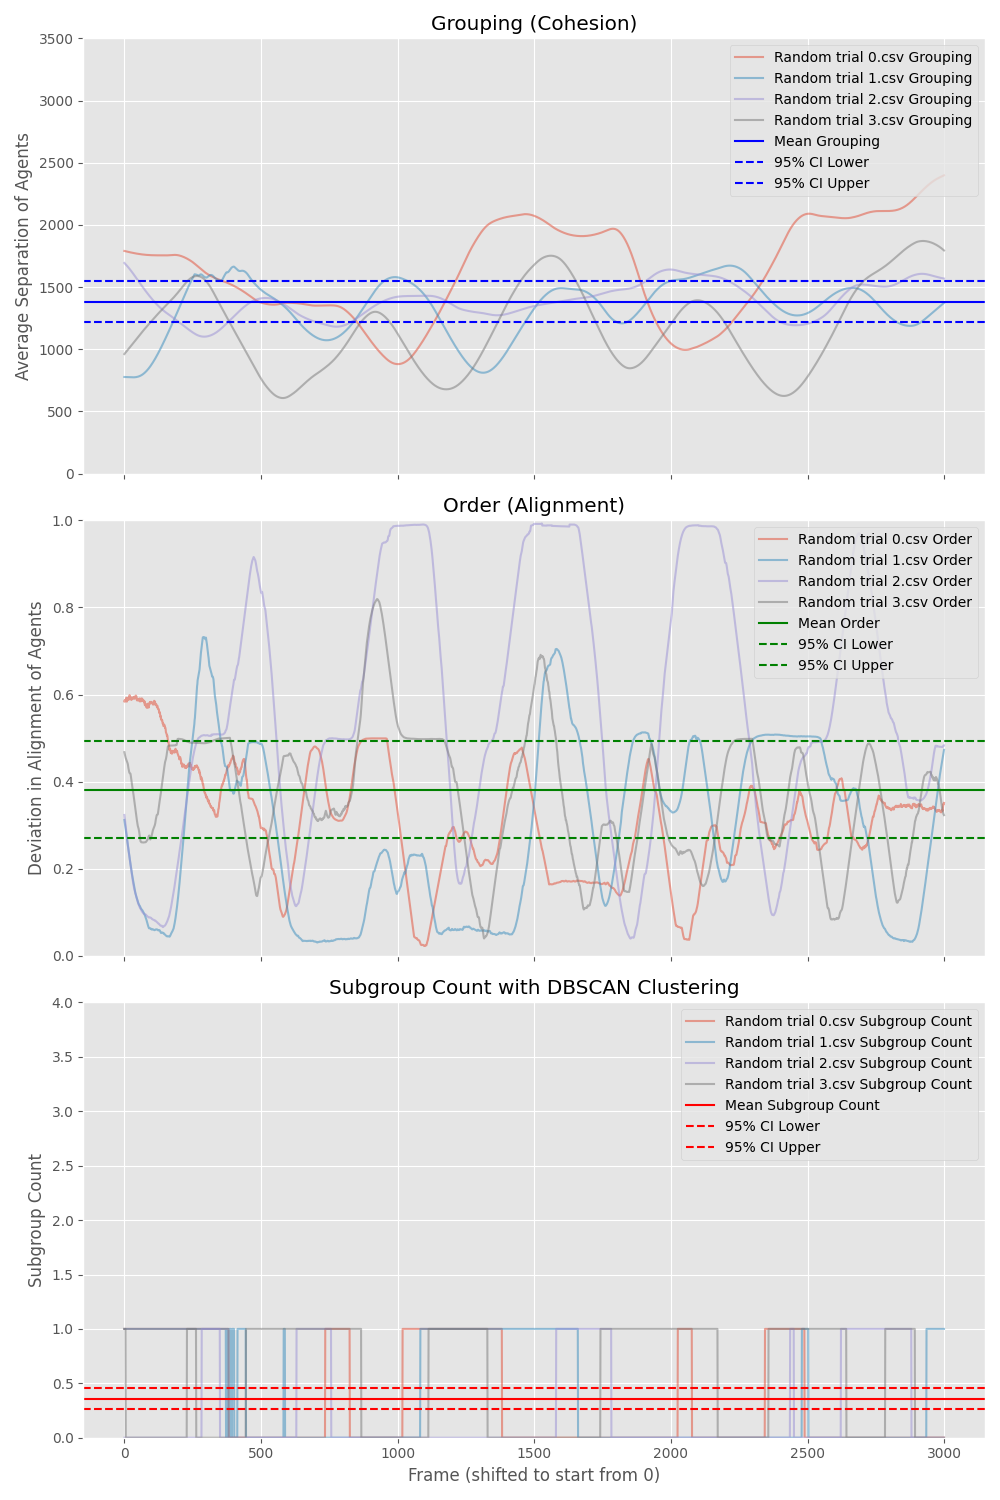
\includegraphics[width=0.45\textwidth]{combined_trials/Random CI Comparison.png}
        \caption{Metrics for Random, depicting mean and 95\% confidence interval of Grouping, Order and Subgroup Count across four trials}
        \label{fig:brownian_metrics}
    \end{figure}

Random motion as a behaviour is characterised by complete irregularity with no swarming, all of the Boid parameters are set to zero and robots move by reflecting within a bounded box, this can be observed in figure \ref{fig:brownian_plot}. The metrics gathered from this run provide a control variable to compare the emergent behaviours against, showing that the behaviours emerge from the Boid swarming parameters and are not simply artefacts of stochastic movement.

By observing the metrics in figure \ref{fig:brownian_metrics} it can be observed that there is a consistently high grouping, due to a large separation between agents, low order, due to a no alignment weight and low subgroup count as no swarms are formed at all.  
\subsection{Flocking}

    \begin{figure}[htbp]
        \centering
        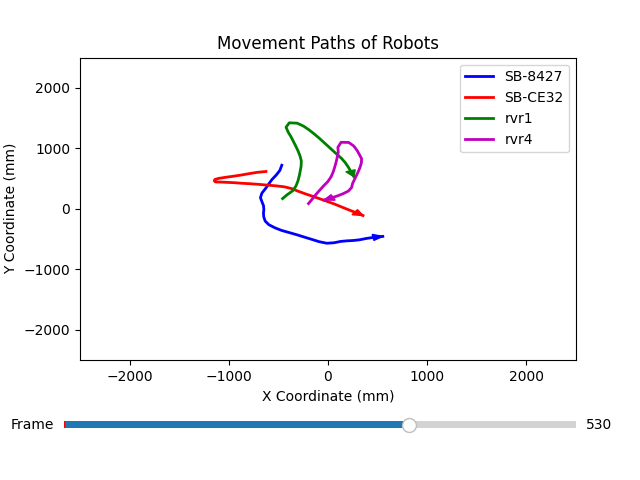
\includegraphics[width=0.45\textwidth]{location_plots/flocking.png}
        \caption{Flocking Behaviour Movement Paths, each colour corresponds to a separate agent within the swarm}
        \label{fig:flocking_plot}
    \end{figure}
    \begin{figure}[htbp]
        \centering
        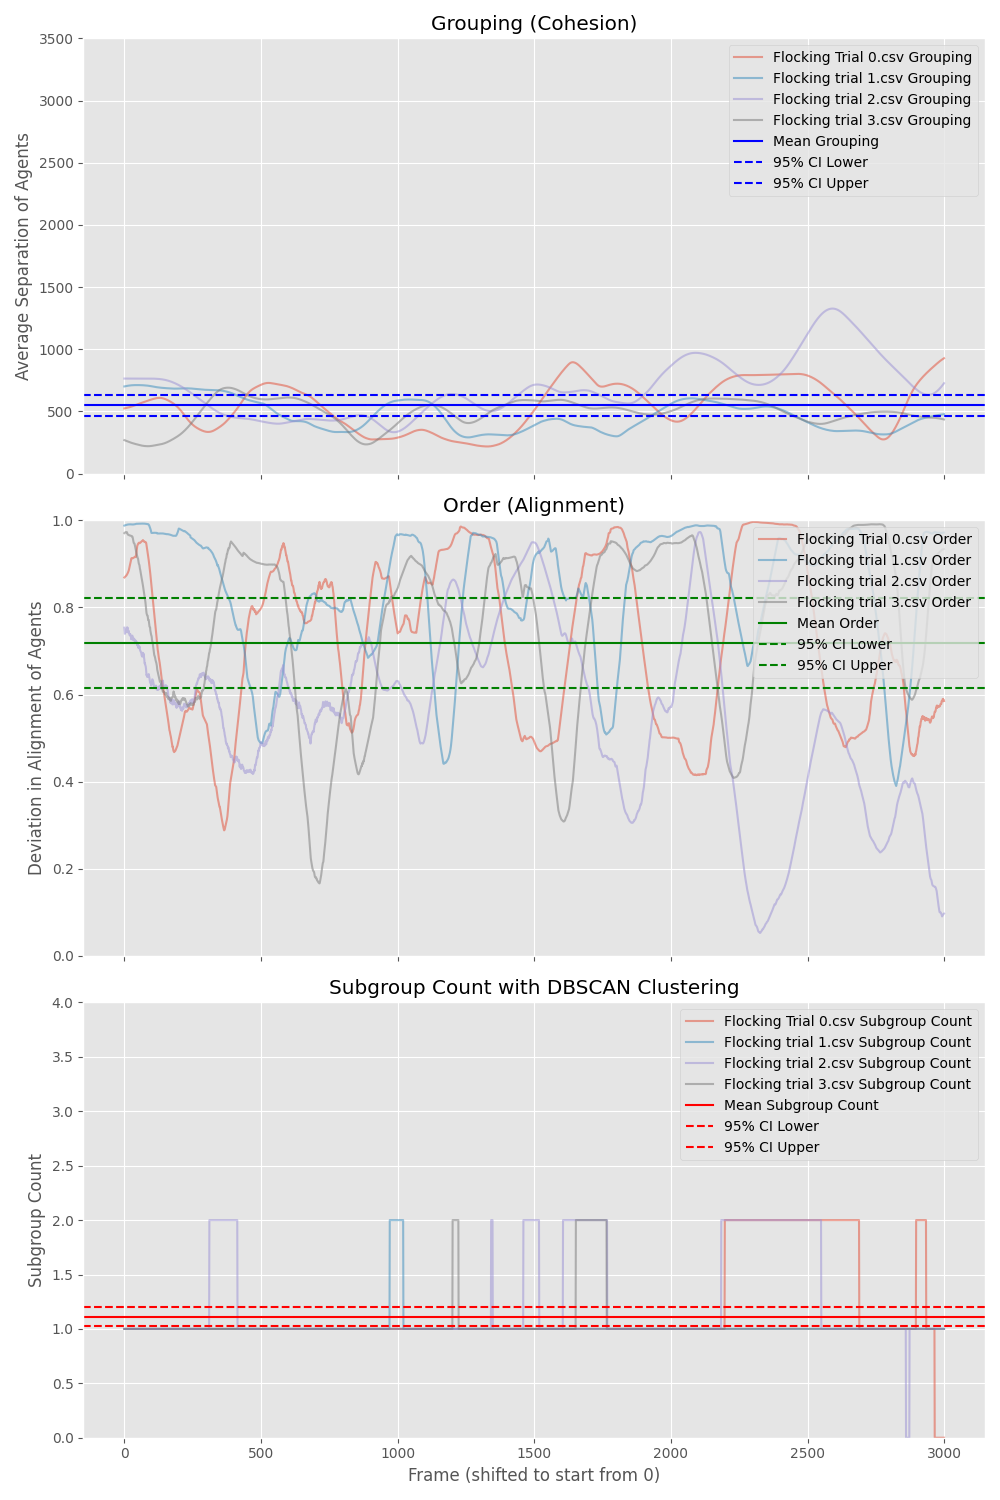
\includegraphics[width=0.45\textwidth]{combined_trials/Flocking CI Comparison.png}
        \caption{Metrics for Flocking, depicting mean and 95\% confidence interval of Grouping, Order and Subgroup Count across four trials}
        \label{fig:flocking_metrics}
    \end{figure}

Within nature, swarming animals vulnerable to predation often exhibit flocking behaviour to improve their chances of survival. This behaviour creates safety in numbers, making it harder for predators to single out individual members. In a similar fashion, robotic swarms can create scalable and robust flocking behaviour to enhance both efficiency and resilience. 

The flocking behaviour can be observed in figure \ref{fig:flocking_plot}, through analysing the paths it shows four agents moving together and avoiding collisions once close, this can be seen particularly well in this freeze-frame in the path of an RVR (rvr4 - purple) and BOLT (SB-CE32 - red), this shows the targeted behaviour of heterogeneous flocking. The metrics show a significantly increased order and decreased grouping compared to the random motion, these particular distributions seen in figure \ref{fig:flocking_metrics} show that the flocking behaviour is both consistent and robust, resulting in less loss of cohesion and alignment, this is further reflected by the significantly closer to one subgroup count. 
\subsection{Line Following}
    
    \begin{figure}[htbp]
        \centering
        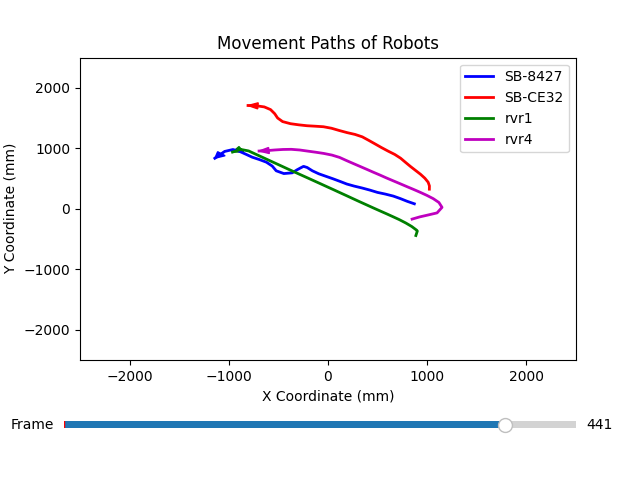
\includegraphics[width=0.45\textwidth]{location_plots/line.png}
        \caption{Line Following Behaviour Movement Paths, each colour corresponds to a separate agent within the swarm}
        \label{fig:line_plot}
    \end{figure}
 
    \begin{figure}[htbp]
        \centering
        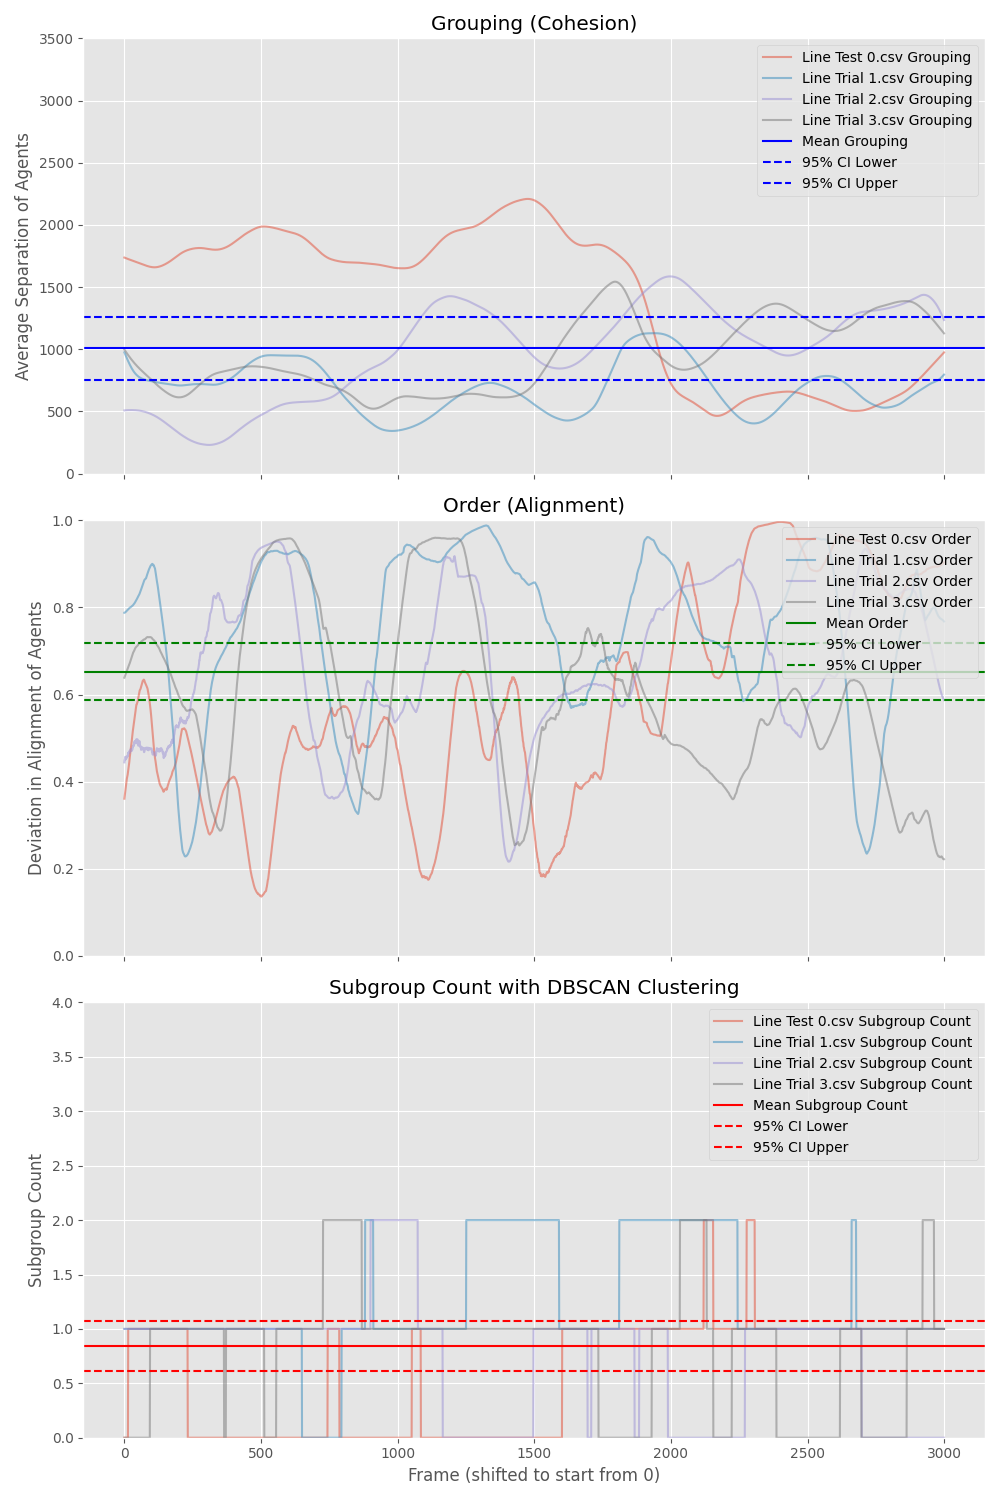
\includegraphics[width=0.45\textwidth]{combined_trials/Line CI Comparison.png}
        \caption{Metrics for Line Following, depicting mean and 95\% confidence interval of Grouping, Order and Subgroup Count across four trials}
        \label{fig:line_metrics}
    \end{figure}

Line-following behaviours within swarms are commonly observed within ants and other insects, these emergent behaviours allow for an efficient logistical system. This can be harnessed within a robotic swarm to serve as both a method of travel and transport of items. 

A line following behaviour can be observed in figure \ref{fig:line_plot}, it can be seen that three agents merge into a distinct line while the BOLT SB-CE32 strays, this is most likely due to the 180-degree field of view utilised in the parameters, this produced strong line following behaviour however this caused any delay in velocity calculation to result in deviation due to slow calculation time. Through analysing the metrics it can be observed in figure \ref{fig:line_metrics} that the grouping mean is significantly below the random mean, while order and subgroup count means are significantly above the random mean, furthermore a high variance in both subgroup count and grouping can be observed, this is most likely due to the swarm losing different elements of the "line, with slower updating of velocities coupled with the restricted field of vision (180 degrees) resulting in more commonly lost groups. 
    
\subsection{Gravity}

    \begin{figure}[htbp]
        \centering
        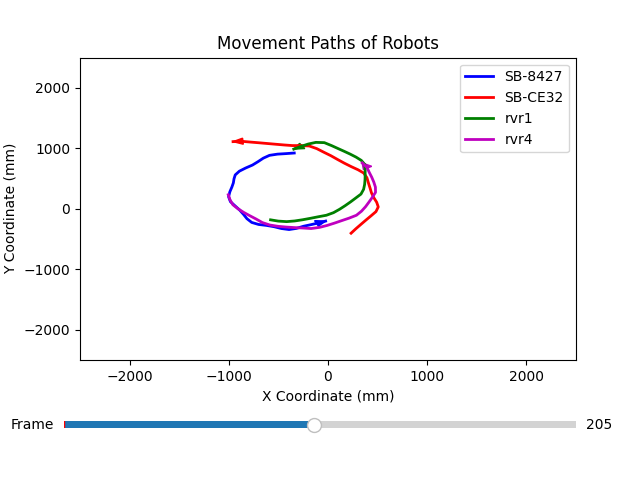
\includegraphics[width=0.45\textwidth]{location_plots/gravity.png}
        \caption{Gravity Behaviour Movement Paths, each colour corresponds to a separate agent within the swarm}
        \label{fig:gravity_plot}
    \end{figure}
 
    \begin{figure}[htbp]
        \centering
        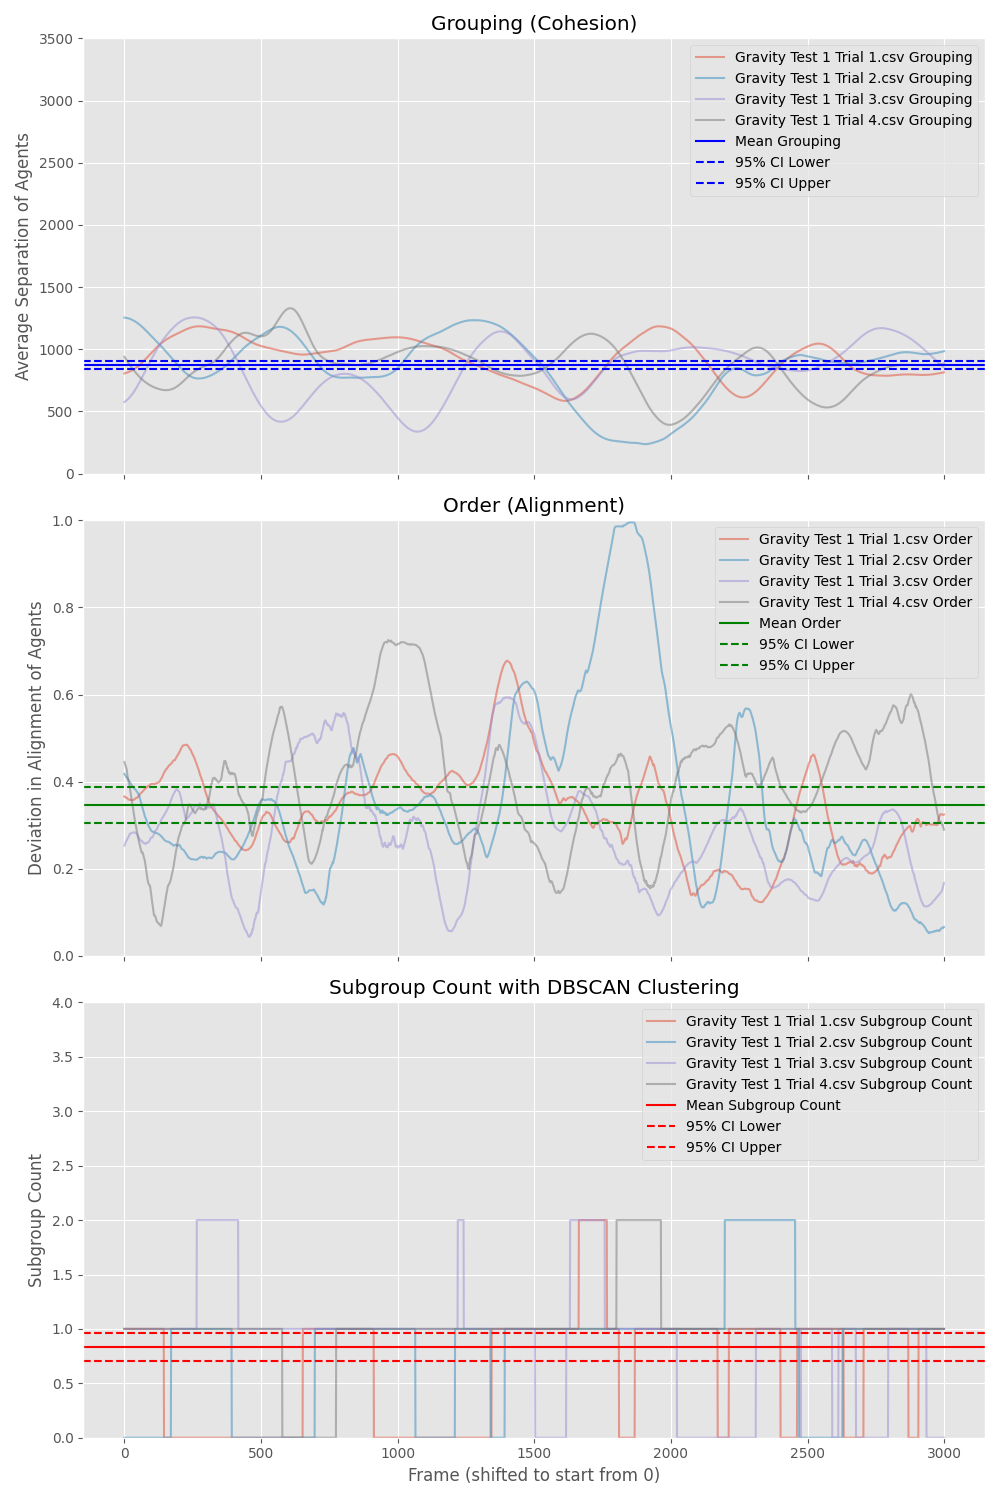
\includegraphics[width=0.45\textwidth]{combined_trials/Gravity CI Comparison.png}
        \caption{Metrics for Gravity, depicting mean and 95\% confidence interval of Grouping, Order and Subgroup Count across four trials}
        \label{fig:gravity_metrics}
    \end{figure}

Predatory animals that hunt in packs typically utilise some form of orbiting, gravity-like behaviour to observe prey while hunting, this allows them to thoroughly assess their environment as well as hold in place. This emergent behaviour within robotic swarms could see applications for surveillance as well as holding patterns for aircraft, with enhanced robustness over a traditional controlled formation as the behaviour is emergent in nature.

A gravity behaviour can be observed in figure \ref{fig:gravity_plot}, this shows all robots travelling continuously in a circle around a central point, thus the desired behaviour has emerged from the parameters utilised. The analysed metrics within figure \ref{fig:gravity_metrics} show the significantly decreased grouping and decreased variance within the grouping showing that the behaviour creates a strong and cohesive group that readily maintains its formation. The order is notably lesser than that of the other emergent behaviours within this report, this is referred to above in Equation \ref{eq:order}; order is a measure of the alignment of headings of all agents and as this behaviour creates a circular structure the agents do not typically face the same way.
\FloatBarrier
\subsection{Summary of Results}

The results from each of the trials demonstrated the distinct collective emergent behaviours of the heterogeneous BOLT and RVR swarms. The characteristics of these behaviours can be observed through the comparative analysis of each metric against the control, this is depicted within figure \ref{fig:results_summary} and table \ref{tab2}. 

\begin{figure}[htbp]
    \centering
    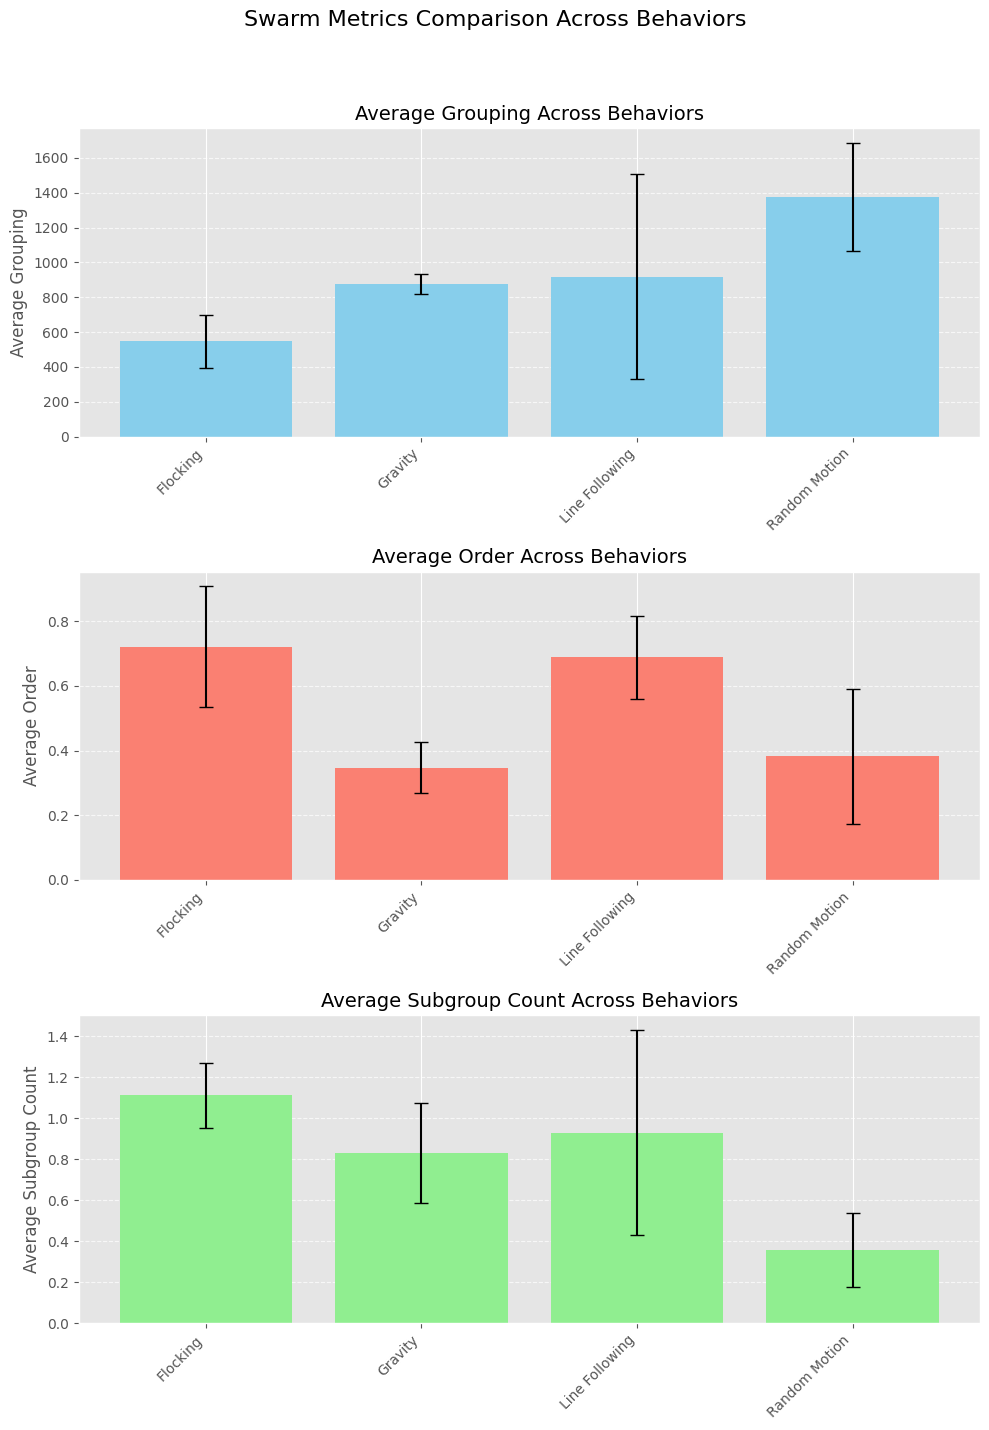
\includegraphics[width=0.45\textwidth]{results_summary_plot.png}
    \caption{Comparison of Metrics of each studied Behaviour with a 95\% Confidence Interval}
    \label{fig:results_summary}
\end{figure}

\begin{table}[h]
\centering
\caption{Studied Behaviours Metrics Mean with a 95\% Confidence Interval}
\label{tab2}
\begin{tabularx}{\columnwidth}[h]{|X|X|X|X|}
\hline
\textbf{Behaviour} & \textbf{Grouping ($\mu \pm$ CI)} & \textbf{Order ($\mu \pm$ CI)} & \textbf{Subgroup Count ($\mu \pm$ CI)} \\ \hline
Flocking          & 546.79 $\pm$ 153.90        & 0.72 $\pm$ 0.19       & 1.11 $\pm$ 0.16         \\ \hline
Gravity           & 875.46 $\pm$ 56.76         & 0.35 $\pm$ 0.08       & 0.83 $\pm$ 0.24         \\ \hline
Line Following    & 919.21 $\pm$ 589.50        & 0.69 $\pm$ 0.13       & 0.93 $\pm$ 0.50         \\ \hline
Random Motion     & 1375.68 $\pm$ 310.40       & 0.38 $\pm$ 0.21       & 0.36 $\pm$ 0.18         \\ \hline %
\end{tabularx}
\end{table}

 As the observed metrics exceeded the 95\% confidence interval for random motion it can be determined that each swarming behaviour is unique and distinct, further insight can be gained from the comparative analysis of each of the metrics: 
\begin{itemize}

    \item The \textbf{grouping} for each behaviour is significantly lower than the control variable, this indicates that each behaviour brings agents together, decreasing their separation. An observed irregularity within these results is the larger variance for the line-following behaviour, which has emerged due to instances of robots becoming lost from the swarm due to a reduced view angle.
    
    \item The \textbf{order} for each behaviour showed statistical differences against the control variable, with all behaviours exhibiting lower variance, flocking and line following have a significantly higher mean order, this indicates that both behaviours result in robots becoming more aligned with each other, while the lower mean order of gravity represents the circular motion resulting in no alignment.

    \item The \textbf{subgroup count} showed that across each behaviour the robots did not quickly disperse apart as all behaviours have mean subgroup counts close to one, which indicates only one group of robots and thus the swarm staying together. Furthermore, it can be observed that each of the studied emergent behaviours showed significantly higher mean subgroup counts than the control, this is because the random behaviour does not bring groups together so does not successfully form any subgroups at all.
    
\end{itemize}

Hence through the analysis of the metrics of grouping, order and subgroup count, valuable insight has been gained into the cohesion, alignment and separation of the swarm. These results thus demonstrate how the adjustment and tuning of Boid parameters can induce specific emergent behaviours in heterogeneous robotic swarms, with each of the emergent behaviours produced above showing real-world applications. 

\FloatBarrier
\section{Conclusion}

This project demonstrated a successful implementation of emergent behaviours within a heterogeneous swarm utilising the low-cost, accessible platforms of Sphero RVR and BOLT robots. This was achieved through the use of a centralised swarm controller that operated each agent in an individual decentralised framework, this was done due to significant challenges within the initial decentralised approach, which ultimately failed due to hardware limitations. Thus, through the integration of the Boid swarming model into a heterogeneous robotic swarm key emergent behaviours such as flocking, line following and gravity-like orbiting were observed, recorded and analysed, these experimental results validated the emergent behaviours and parameters used. This work lays a strong foundation for further research into heterogeneous swarming as the hand-tuned emergent behaviours proposed in this project can be used as a basis for reinforcement learning for automatically tuning emergent behaviours in heterogeneous swarms, while further research into this area could experiment with the application of the swarm to a task, such as gas source localisation or exploration.

\newpage

\bibliographystyle{ieeetr}
\bibliography{IEEEabrv,zotero}

\newpage
\FloatBarrier
\section{Appendices}
\small{Note: Swarming Behaviour 1 test 3 data log was corrupted
and could not be used}
\subsection{Parameter Tuning Metrics}
\vspace{2.9cm}
\begin{figure}[htbp]
    \centering
    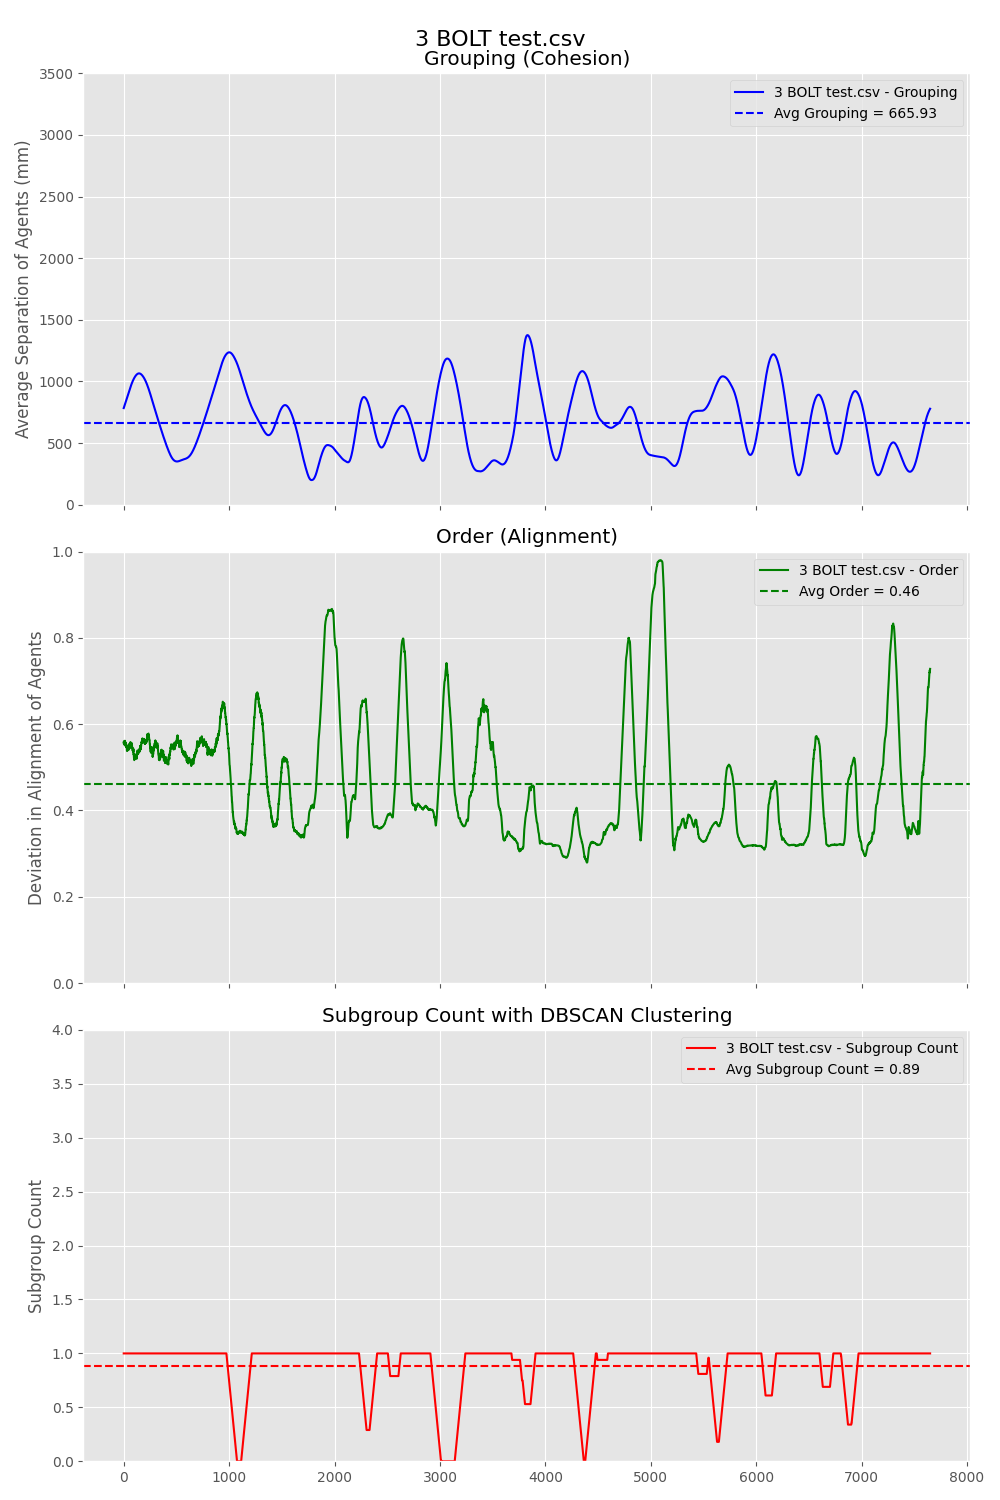
\includegraphics[width=0.45\textwidth]{appendix/3 bolt test.csv metric plot.png}
    \caption{Metrics for 3 Bolt Test}
    \label{fig:3_bolt_test}
\end{figure}

\begin{figure}[htbp]
    \centering
    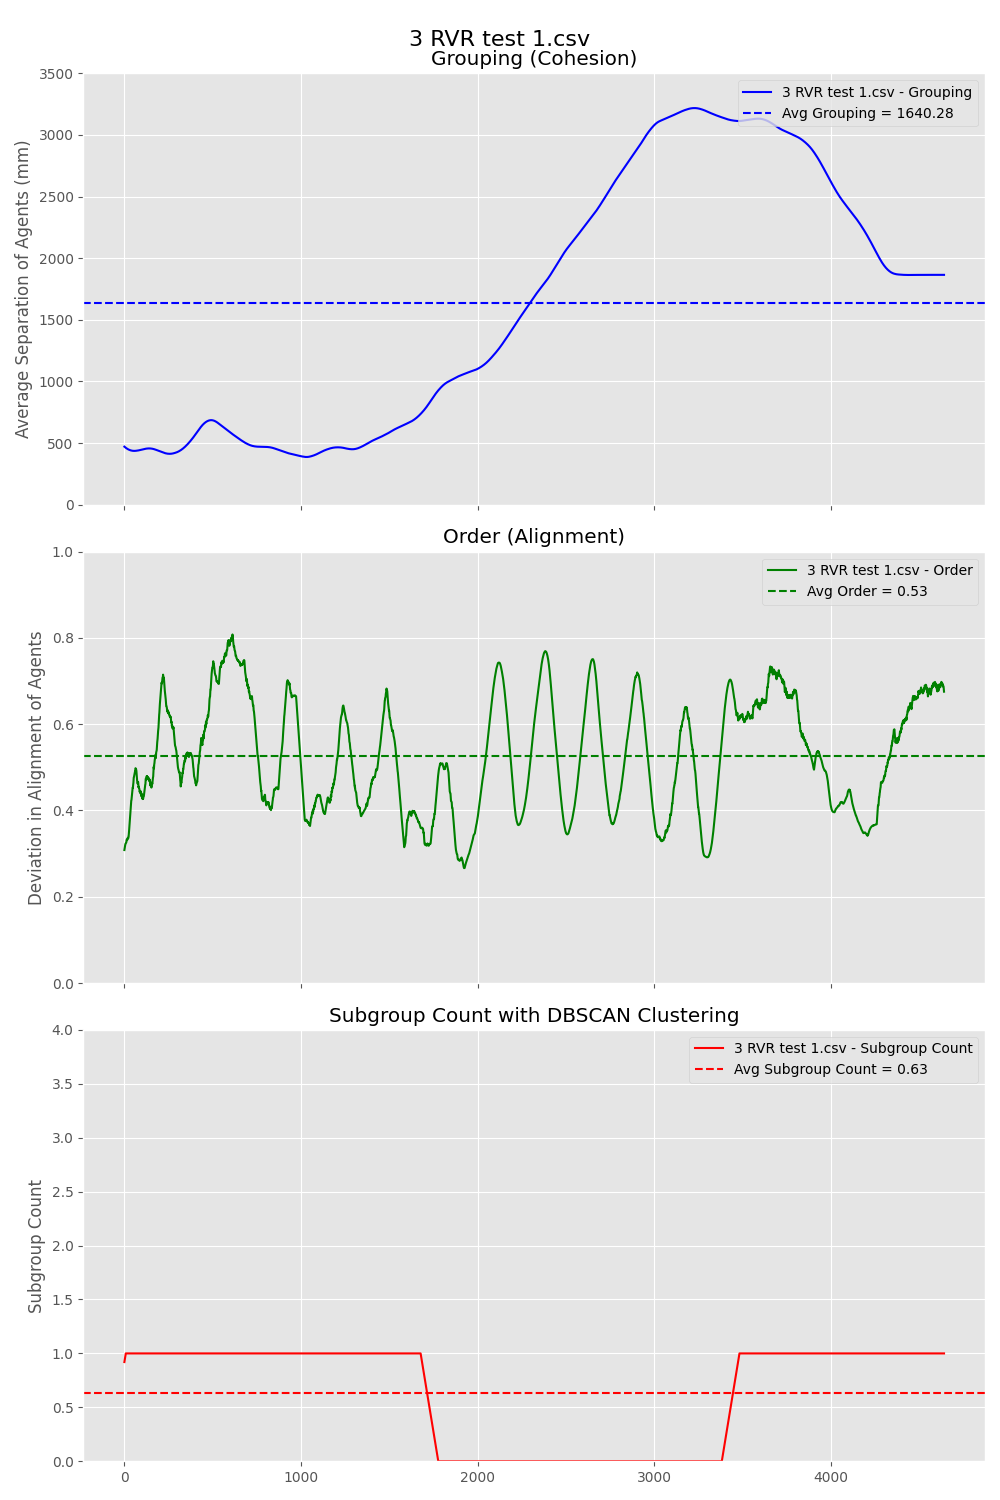
\includegraphics[width=0.45\textwidth]{appendix/3 RVR test 1.csv metric plot.png}
    \caption{Metrics for 3 RVR Test 1}
    \label{fig:3_RVR_test_1}
\end{figure}

\begin{figure}[htbp]
    \centering
    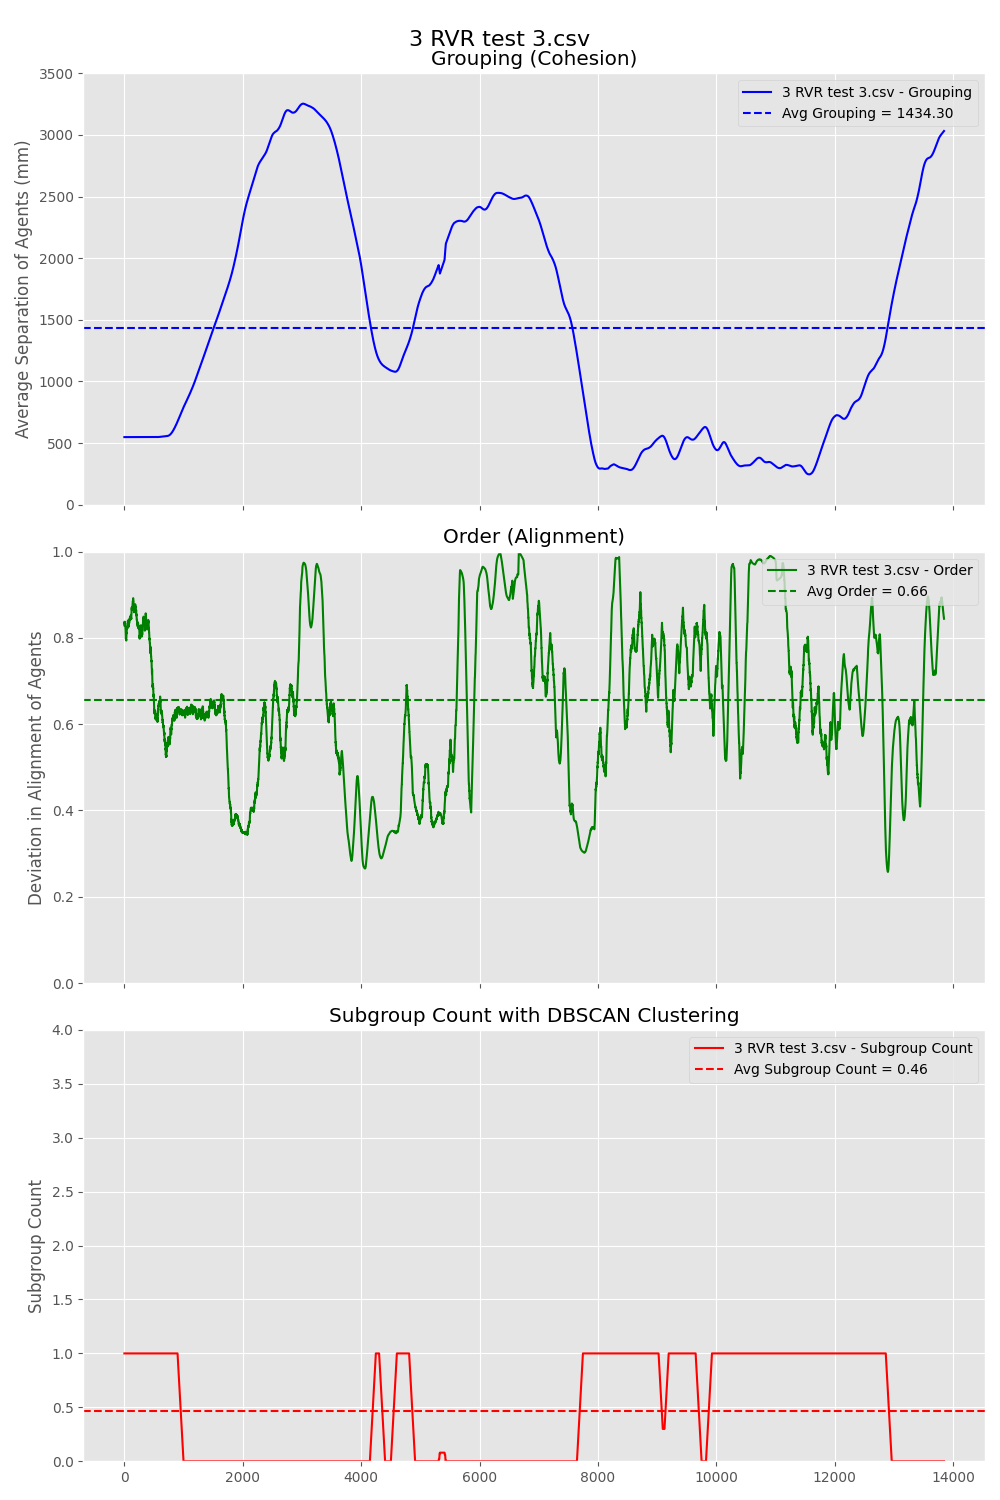
\includegraphics[width=0.45\textwidth]{appendix/3 RVR test 3.csv metric plot.png}
    \caption{Metrics for Homogeneous three RVR Test 3}
    \label{fig:3_RVR_test_3}
\end{figure}

\begin{figure}[htbp]
    \centering
    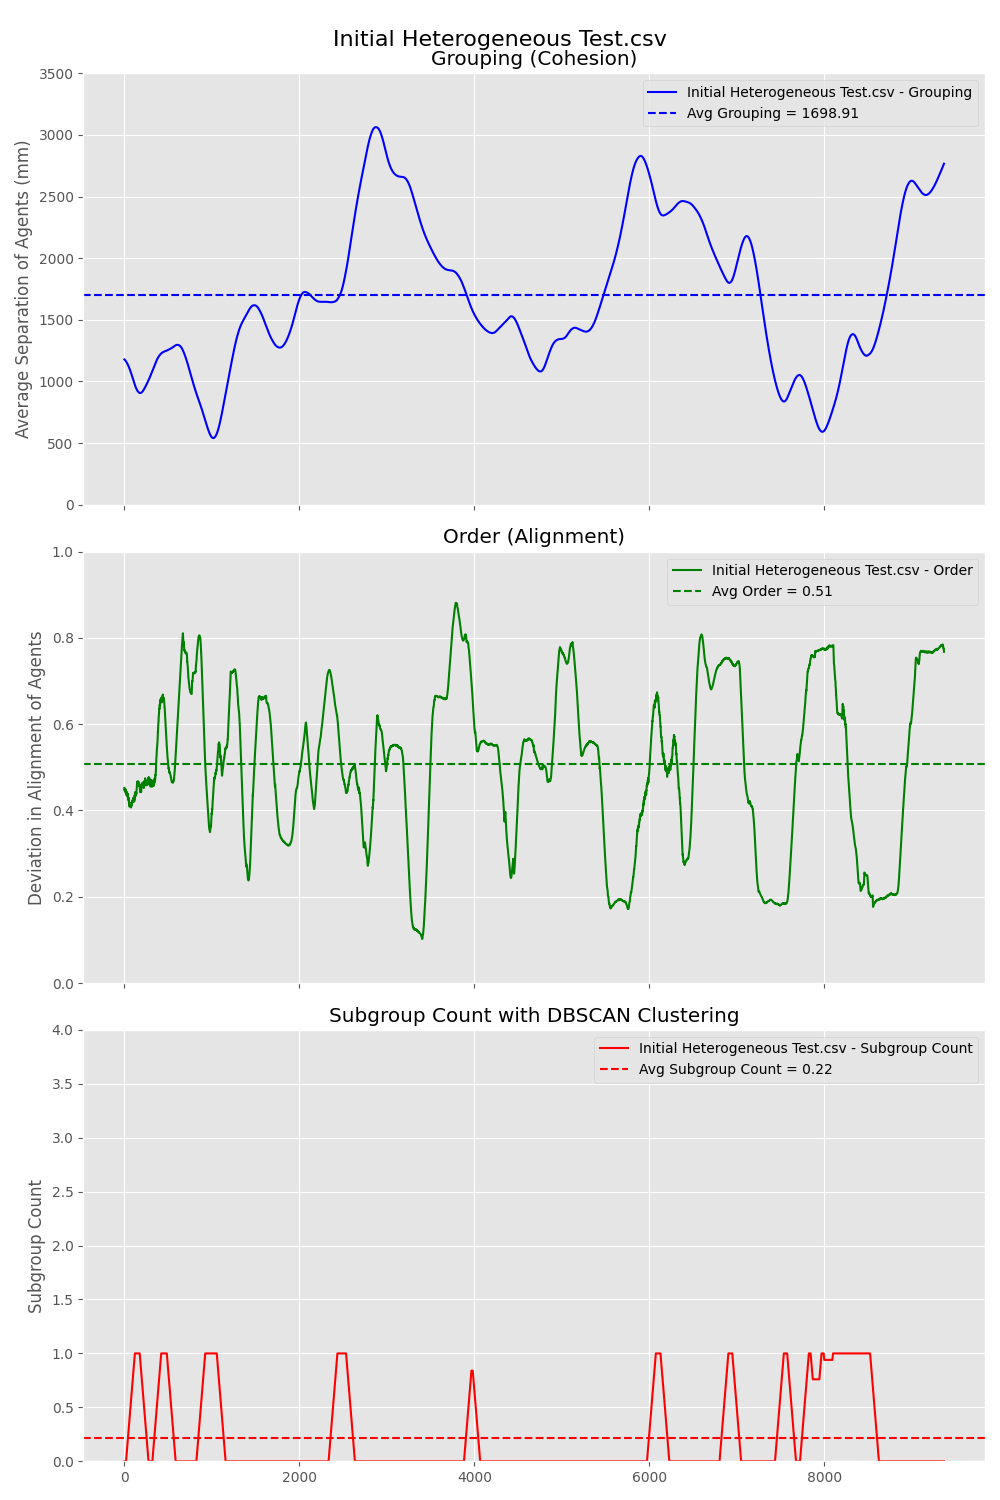
\includegraphics[width=0.45\textwidth]{appendix/Initial Heterogeneous Test.csv metric plot.png}
    \caption{Metrics for Initial Heterogeneous Test}
    \label{fig:hetero_test_3}
\end{figure}

\begin{figure}[htbp]
    \centering
    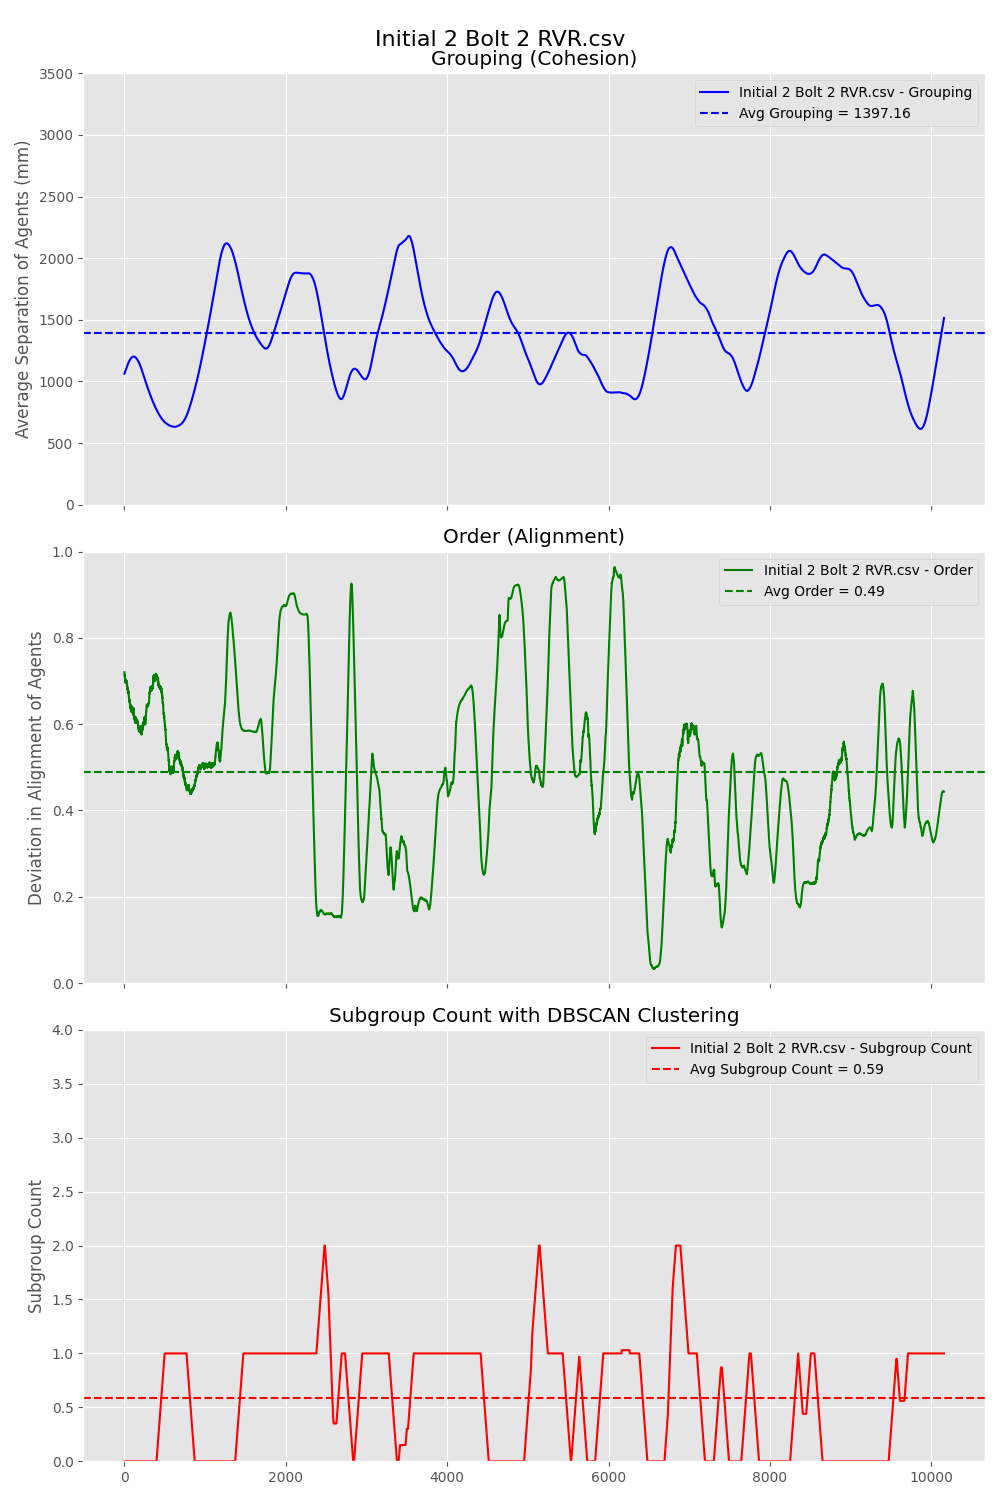
\includegraphics[width=0.45\textwidth]{appendix/Initial 2 Bolt 2 RVR.csv metric plot.png}
    \caption{Metrics for Initial 2 Bolt 2 RVR}
    \label{fig:initial_2_bolt_2_rvr}
\end{figure}

\begin{figure}[htbp]
    \centering
    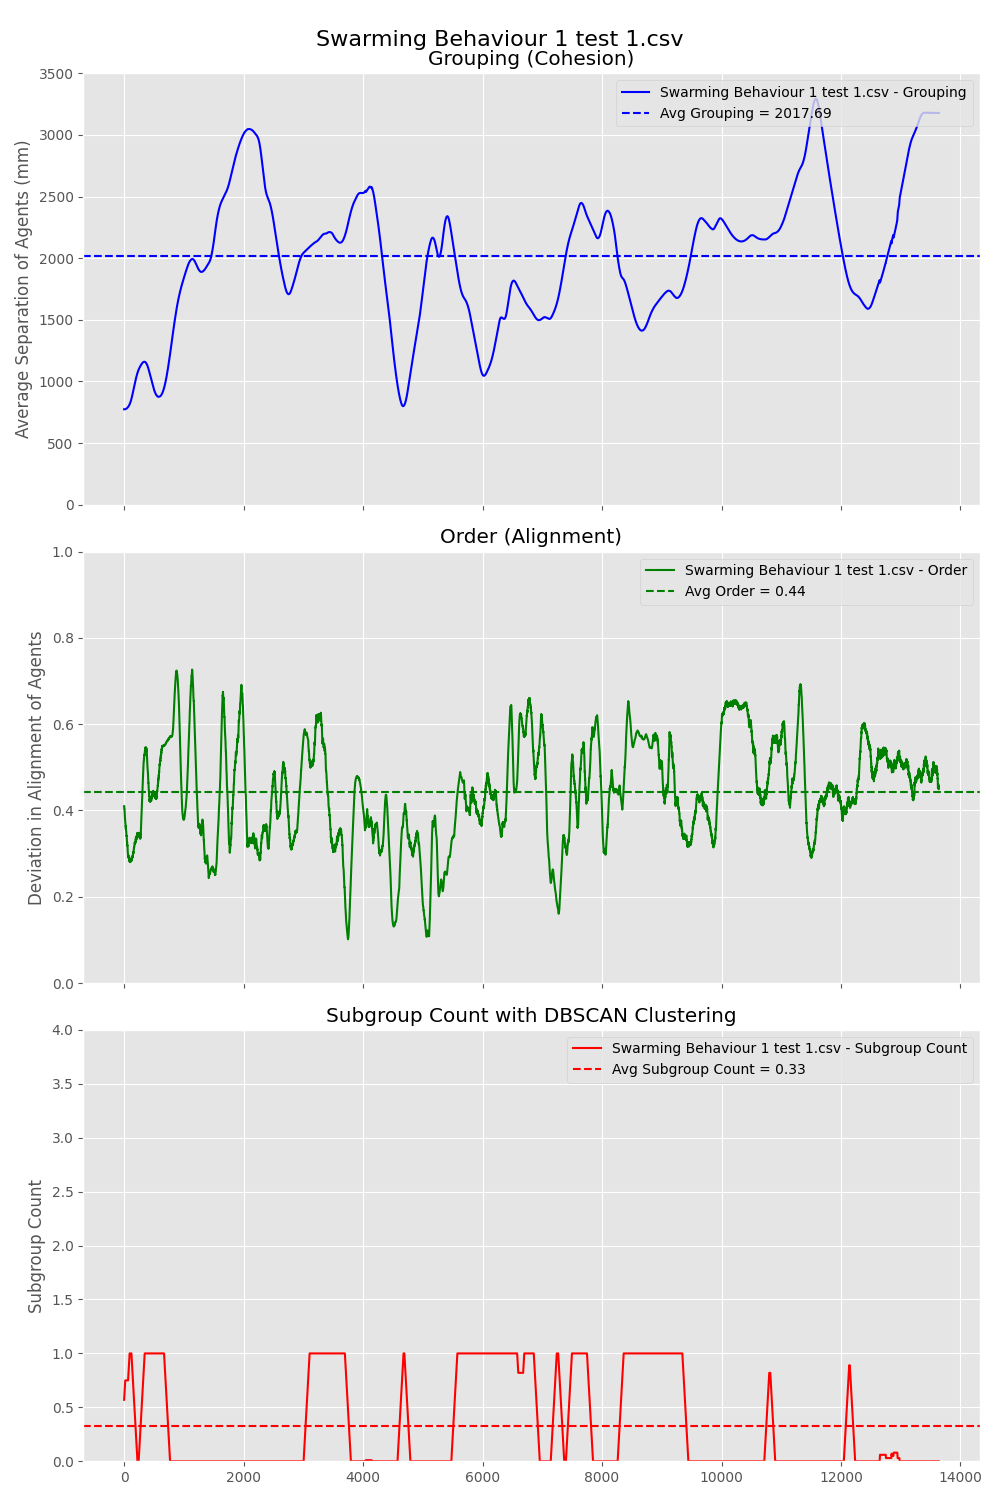
\includegraphics[width=0.45\textwidth]{appendix/Swarming Behaviour 1 test 1.csv metric plot.png}
    \caption{Metrics for Swarming Behaviour 1 Test 1}
    \label{fig:swarming_behaviour_1_test_1}
\end{figure}

\begin{figure}[htbp]
    \centering
    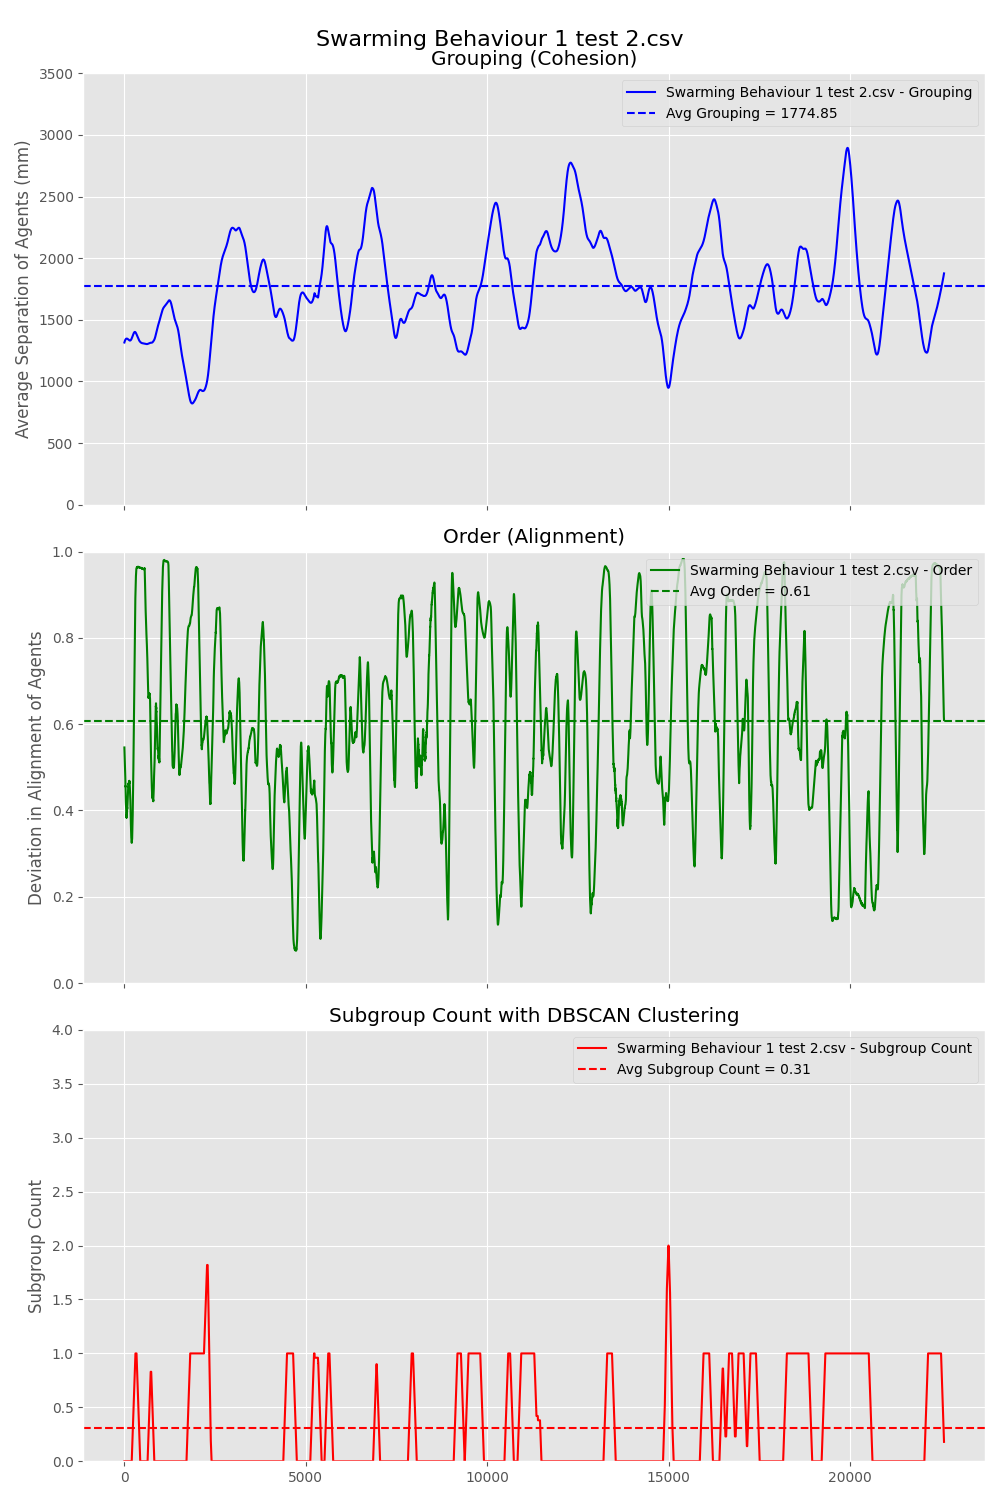
\includegraphics[width=0.45\textwidth]{appendix/Swarming Behaviour 1 test 2.csv metric plot.png}
    \caption{Metrics for Swarming Behaviour 1 Test 2}
    \label{fig:swarming_behaviour_1_test_2}
\end{figure}

\begin{figure}[htbp]
    \centering
    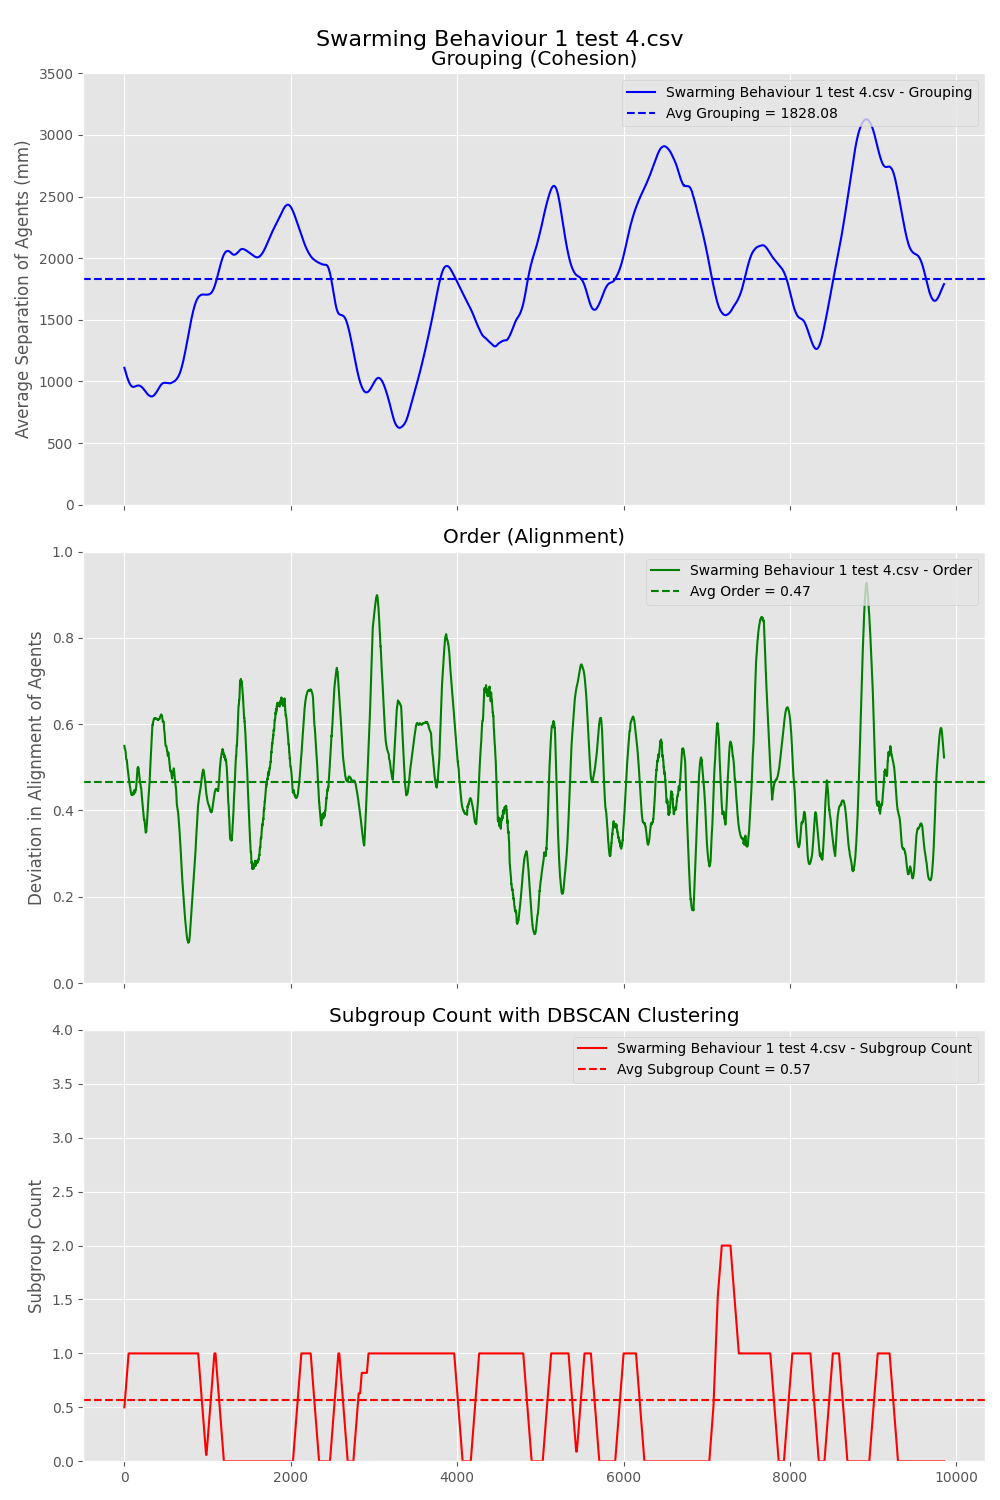
\includegraphics[width=0.45\textwidth]{appendix/Swarming Behaviour 1 test 4.csv metric plot.png}
    \caption{Metrics for Swarming Behaviour 1 Test 4}
    \label{fig:swarming_behaviour_1_test_4}
\end{figure}

\begin{figure}[htbp]
    \centering
    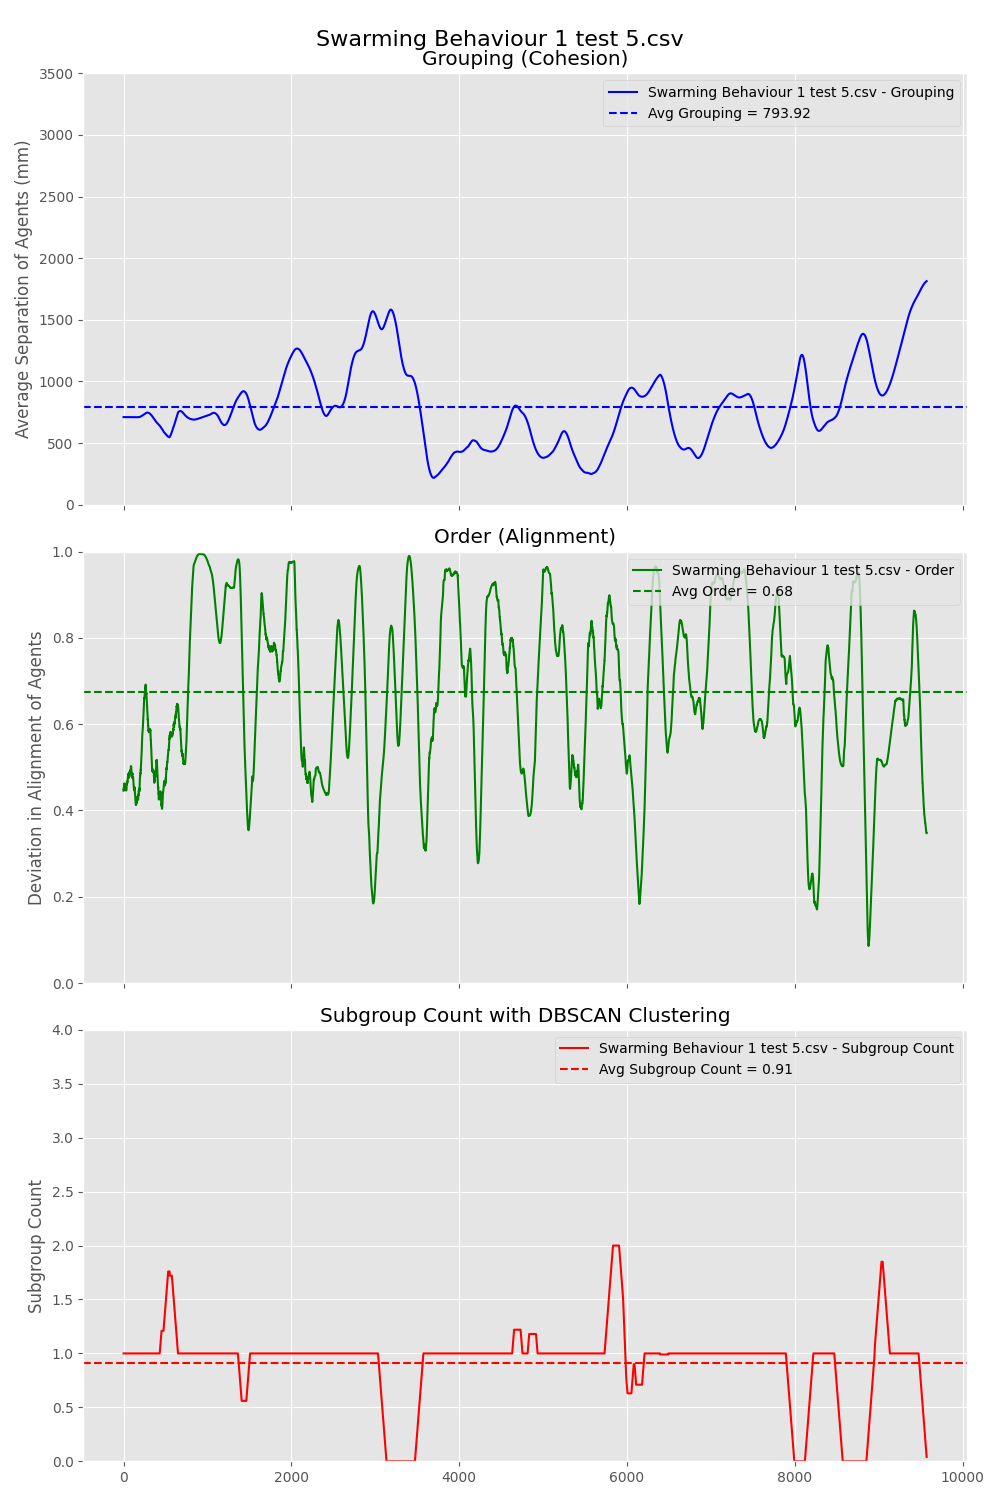
\includegraphics[width=0.45\textwidth]{appendix/Swarming Behaviour 1 test 5.csv metric plot.png}
    \caption{Metrics for Swarming Behaviour 1 Test 5}
    \label{fig:swarming_behaviour_1_test_5}
\end{figure}

\begin{figure}[htbp]
    \centering
    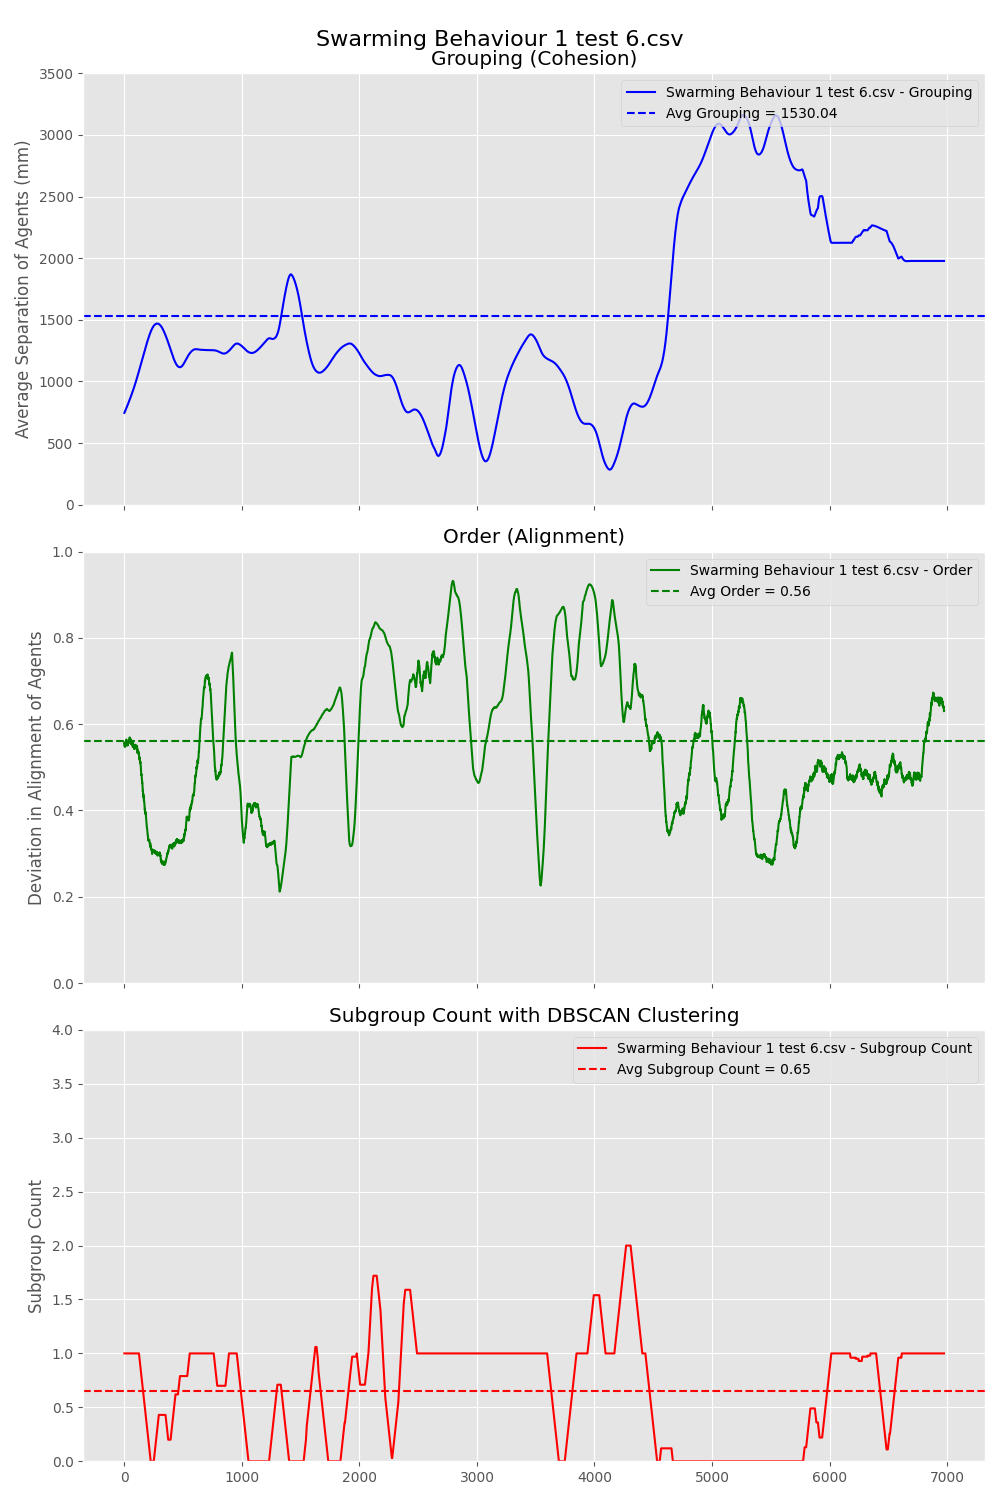
\includegraphics[width=0.45\textwidth]{appendix/Swarming Behaviour 1 test 6.csv metric plot.png}
    \caption{Metrics for Swarming Behaviour 1 Test 6}
    \label{fig:swarming_behaviour_1_test_6}
\end{figure}

\begin{figure}[htbp]
    \centering
    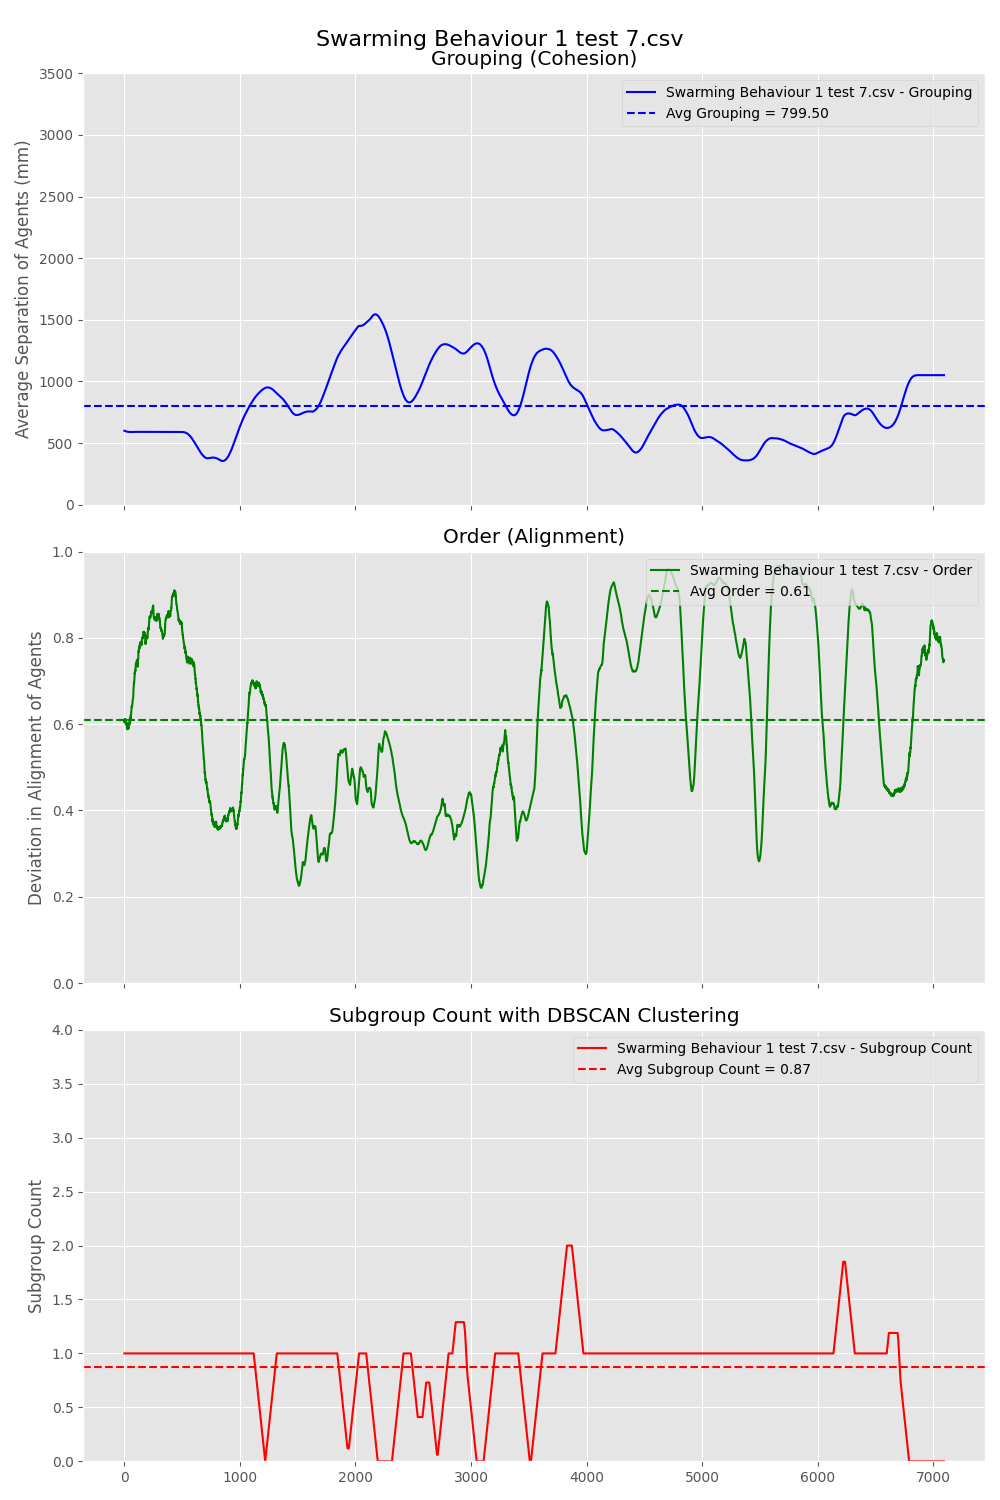
\includegraphics[width=0.45\textwidth]{appendix/Swarming Behaviour 1 test 7.csv metric plot.png}
    \caption{Metrics for Swarming Behaviour 1 Test 7}
    \label{fig:swarming_behaviour_1_test_7}
\end{figure}

\begin{figure}[htbp]
    \centering
    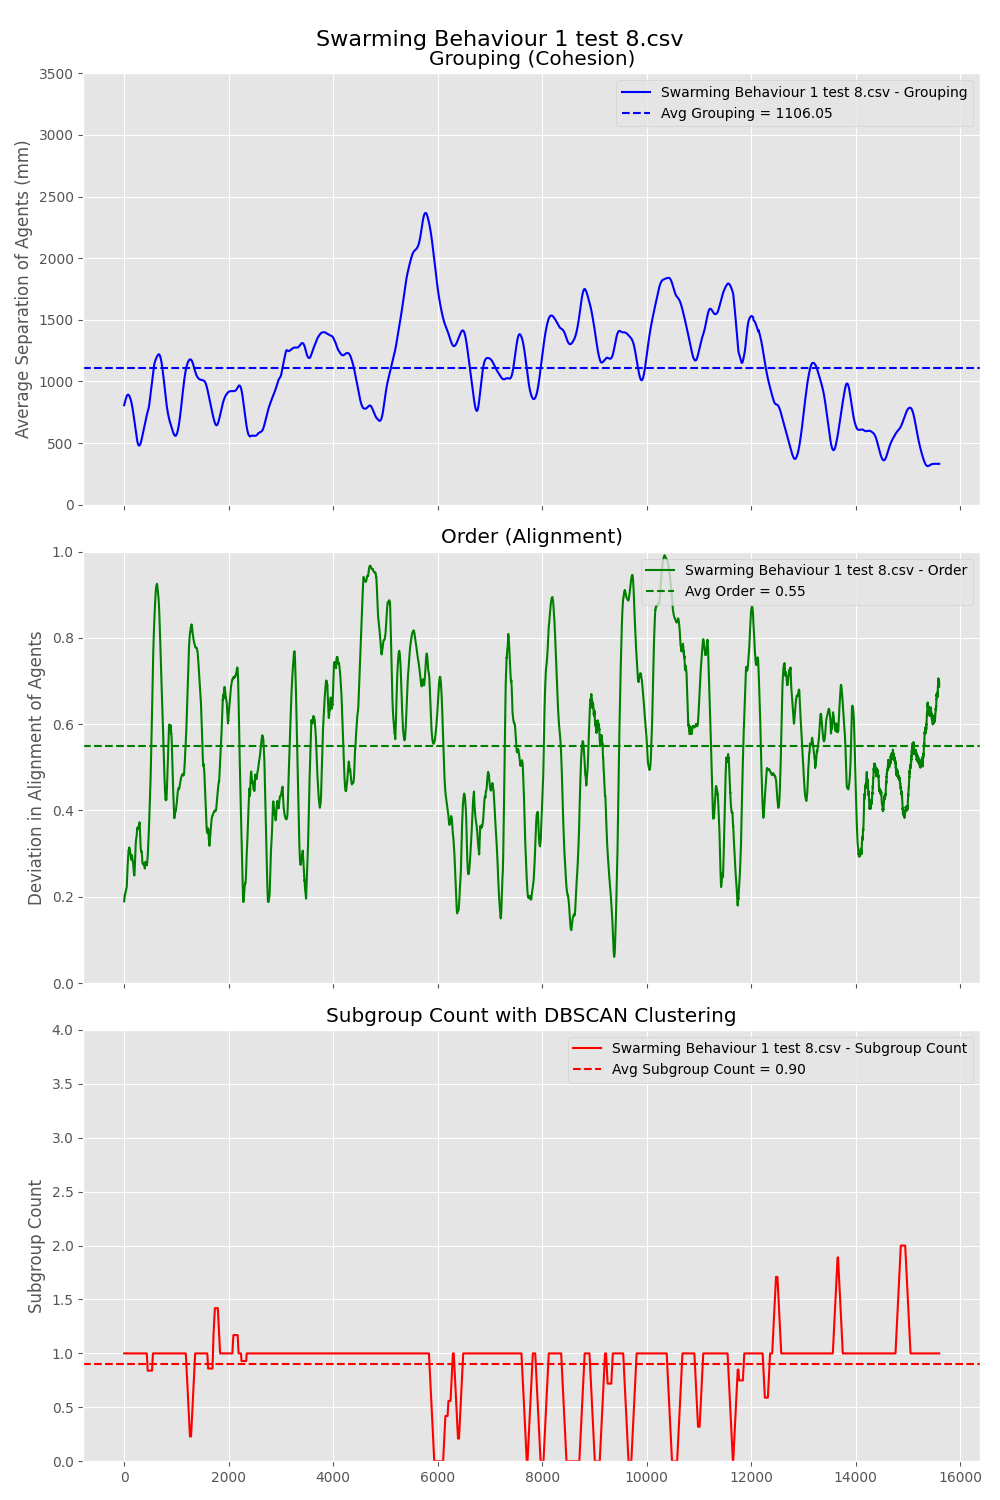
\includegraphics[width=0.45\textwidth]{appendix/Swarming Behaviour 1 test 8.csv metric plot.png}
    \caption{Metrics for Swarming Behaviour 1 Test 8}
    \label{fig:swarming_behaviour_1_test_8}
\end{figure}

\begin{figure}[htbp]
    \centering
    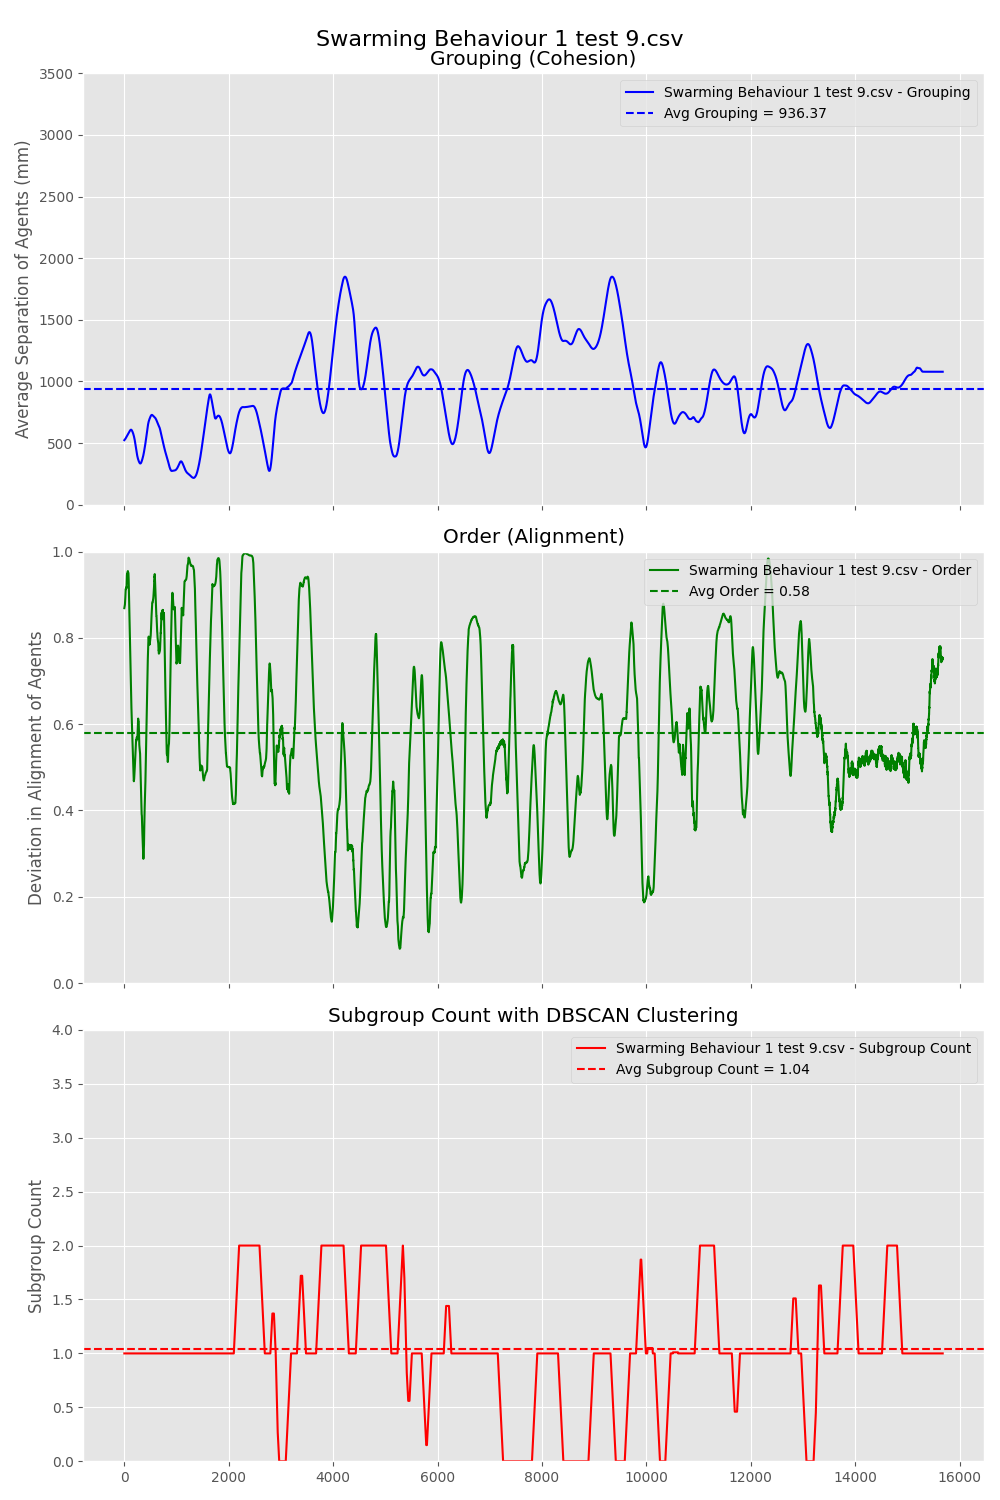
\includegraphics[width=0.45\textwidth]{appendix/Swarming Behaviour 1 test 9.csv metric plot.png}
    \caption{Metrics for Swarming Behaviour 1 Test 9}
    \label{fig:swarming_behaviour_1_test_9}
\end{figure}

\begin{figure}[htbp]
    \centering
    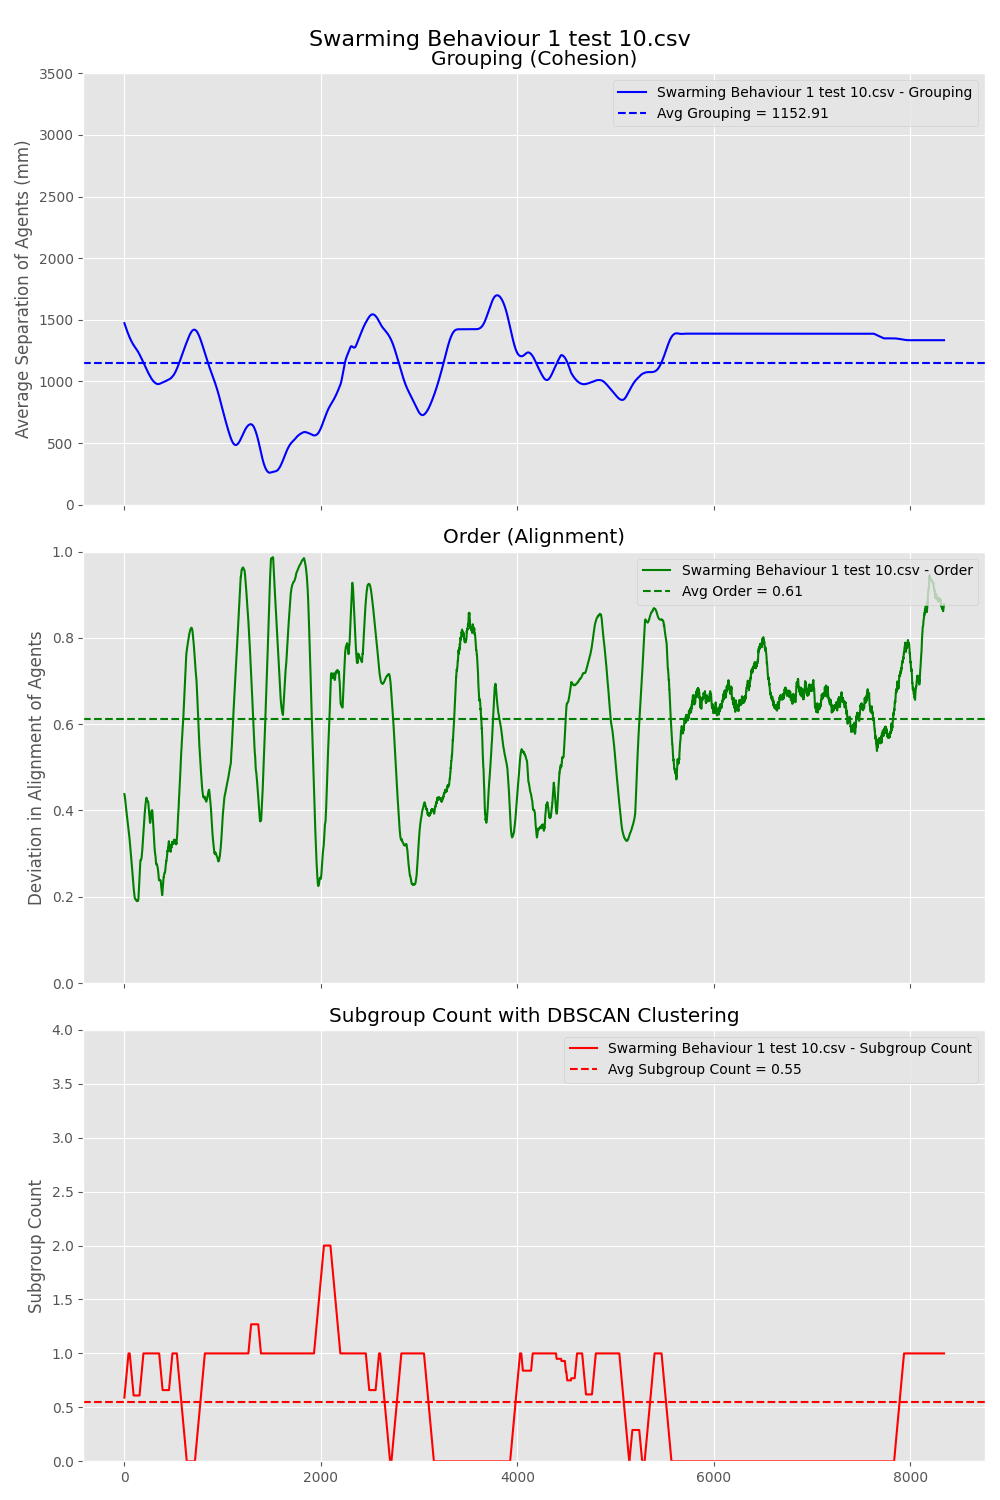
\includegraphics[width=0.45\textwidth]{appendix/Swarming Behaviour 1 test 10.csv metric plot.png}
    \caption{Metrics for Swarming Behaviour 1 Test 10}
    \label{fig:swarming_behaviour_1_test_10}
\end{figure}

\begin{figure}[htbp]
    \centering
    
\includegraphics[width=0.45\textwidth]{appendix/line test 1.csv metric plot.png}
    \caption{Metrics for Line Test 1}
    \label{fig:line_test_1}
\end{figure}

\onecolumn
\FloatBarrier
\subsection{Parameters for Tuning and Validation Studies}

\begin{table*} [htbp]
    \centering
    \caption{Parameters used during parameter tuning and validation studies}
    \begin{tabular}{|c|c|c|c|c|c|c|c|c|c|c|}
    \hline
        \textbf{Test Name} & \textbf{Robot} & $\mathbf{R_c}$ & $\mathbf{R_a}$ & $\mathbf{R_s}$ & $\mathbf{W_c}$ & $\mathbf{W_a}$ & $\mathbf{W_s}$ & $\mathbf{\theta_{vision}}$ & $\mathbf{V_{min}}$ & $\mathbf{V_{max}}$ \\ \hline
        \textbf{3 BOLT Test} & BOLT & 100 & 100 & 25 & 0.02 & 0.02 & 0.01 & 360 & 70 & 80 \\ \hline
        \textbf{3 RVR Test} & RVR & 100 & 100 & 25 & 0.02 & 0.02 & 0.01 & 360 & 70 & 80 \\ \hline
        \textbf{Initial Heterogeneous Test} & BOLT & 100 & 100 & 25 & 0.02 & 0.02 & 0.01 & 360 & 70 & 80 \\ \hline
        \textbf{Initial Heterogeneous Test} & RVR & 100 & 100 & 25 & 0.2 & 0.2 & 0.1 & 360 & 70 & 80 \\ \hline
        \textbf{2 BOLT 2 RVR Test} & BOLT & 100 & 100 & 25 & 0.02 & 0.02 & 0.01 & 360 & 70 & 80 \\ \hline
        \textbf{2 BOLT 2 RVR Test} & RVR & 100 & 100 & 25 & 0.02 & 0.02 & 0.01 & 360 & 70 & 80\\ \hline
        \textbf{Swarming Behaviour 1 test 1} & BOLT & 100 & 50 & 25 & 0.3 & 0.8 & 0.1 & 360 & 50 & 70 \\ \hline
        \textbf{Swarming Behaviour 1 test 1} & RVR & 100 & 50 & 25 & 0.3 & 0.8 & 0.1 & 360 & 80 & 100\\ \hline
        \textbf{Swarming Behaviour 1 test 2} & BOLT & 100 & 150 & 25 & 0.3 & 0.8 & 0.1 & 360 & 50 & 70\\ \hline
        \textbf{Swarming Behaviour 1 test 2} & RVR & 100 & 150 & 25 & 0.3 & 0.8 & 0.1 & 360 & 80 & 100\\ \hline
        \textbf{Swarming Behaviour 1 test 3} & BOLT & 100 & 150 & 25 & 1.3 & 1 & 0.3 & 360 & 50 & 70\\ \hline
        \textbf{Swarming Behaviour 1 test 3} & RVR & 100 & 150 & 25 & 0.5 & 0.8 & 0.1 & 360 & 70 & 140\\ \hline
        \textbf{Swarming Behaviour 1 test 4} & BOLT & 100 & 100 & 25 & 0.02 & 0.02 & 0.01 & 360 & 70 & 80\\ \hline
        \textbf{Swarming Behaviour 1 test 4} & RVR & 100 & 100 & 25 & 0.1 & 0.02 & 0.01 & 360 & 70 & 80\\ \hline
        \textbf{Swarming Behaviour 1 test 5} & BOLT & 175 & 100 & 50 & 1.3 & 1 & 0.8 & 360 & 50 & 70\\ \hline
        \textbf{Swarming Behaviour 1 test 5} & RVR & 100 & 150 & 100 & 0.5 & 0.8 & 0.4 & 360 & 75 & 115\\ \hline
        \textbf{Swarming Behaviour 1 test 6} & BOLT & 100 & 50 & 25 & 1 & 1 & 1.5 & 360 & 50 & 75\\ \hline
        \textbf{Swarming Behaviour 1 test 6} & RVR & 100 & 50 & 25 & 1 & 1 & 1.5 & 360 & 135 & 150\\ \hline
        \textbf{Swarming Behaviour 1 test 7} & BOLT & 100 & 50 & 25 & 1 & 1 & 1.5 & 360 & 50 & 75\\ \hline
        \textbf{Swarming Behaviour 1 test 7} & RVR & 100 & 50 & 25 & 1 & 1 & 1.5 & 360 & 75 & 105\\ \hline
        \textbf{Swarming Behaviour 1 test 8} & BOLT & 100 & 50 & 35 & 1 & 1 & 1.7 & 360 & 50 & 75\\ \hline
        \textbf{Swarming Behaviour 1 test 8} & RVR & 100 & 50 & 35 & 1 & 1 & 1.7 & 360 & 75 & 105\\ \hline
        \textbf{Swarming Behaviour 1 test 9} & BOLT & 100 & 75 & 50 & 1 & 1.3 & 1.2 & 360 & 50 & 75\\ \hline
        \textbf{Swarming Behaviour 1 test 9} & RVR & 100 & 50 & 35 & 1 & 1.5 & 1.2 & 360 & 75 & 105\\ \hline
        \textbf{Swarming Behaviour 1 test 10} & BOLT & 100 & 75 & 50 & 1 & 1.3 & 1.2 & 360 & 50 & 75\\ \hline
        \textbf{Swarming Behaviour 1 test 10} & RVR & 100 & 50 & 50 & 1 & 1.5 & 1.2 & 360 & 75 & 105 \\ \hline
        \textbf{Line test 1} & BOLT & 100 & 100 & 25 & 1 & 1 & 0 & 180 & 50 & 75 \\ \hline
        \textbf{Line test 1} & RVR & 100 & 100 & 25 & 1 & 1 & 0 & 180 & 75 & 105 \\ \hline
    \end{tabular}
    \label{tab3}
\end{table*}

\FloatBarrier
\twocolumn

\subsection{Location Plots of Tuning and Validation Studies}

\begin{figure}[htbp]
    \centering
    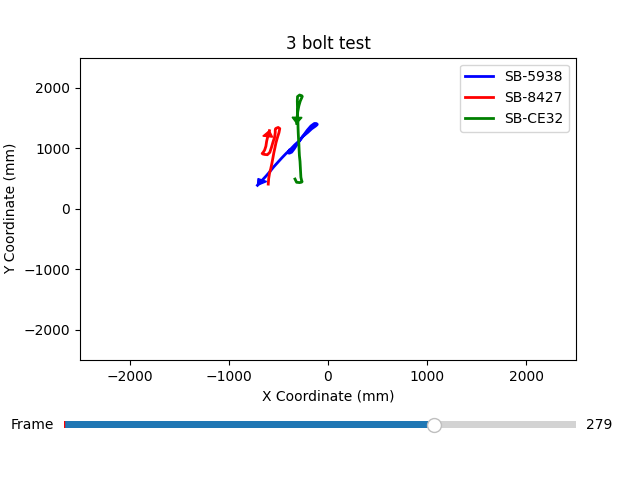
\includegraphics[width=0.4\textwidth]{appendix/3 bolt test plot.png}
    \caption{Location Plot for 3 Bolt Test}
    \label{fig:3_bolt_test_plot}
\end{figure}

\begin{figure}[htbp]
    \centering
    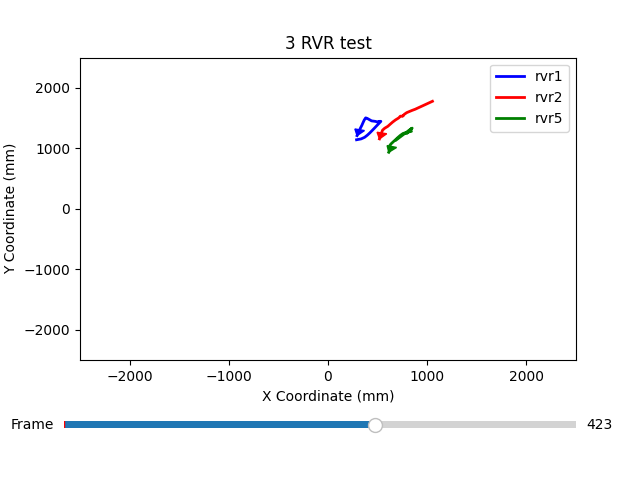
\includegraphics[width=0.4\textwidth]{appendix/3 RVR test.png}
    \caption{Location Plot for 3 RVR test}
    \label{fig:3_RVR_test_3}
\end{figure}

\begin{figure}[htbp]
    \centering
    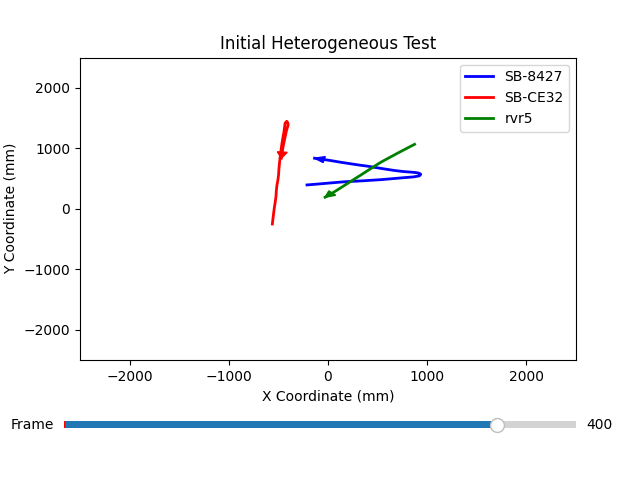
\includegraphics[width=0.4\textwidth]{appendix/Initial Heterogeneous Test plot.png}
    \caption{Location Plot for Initial Heterogeneous Test}
    \label{fig:hetero_test_3}
\end{figure}

\begin{figure}[htbp]
    \centering
    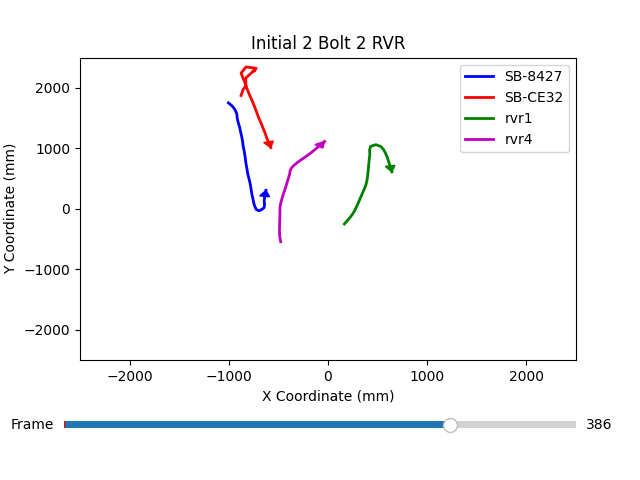
\includegraphics[width=0.4\textwidth]{appendix/Initial 2 Bolt 2 RVR plot.png}
    \caption{Location Plot for Initial 2 Bolt 2 RVR}
    \label{fig:initial_2_bolt_2_rvr}
\end{figure}

\begin{figure}[htbp]
    \centering
    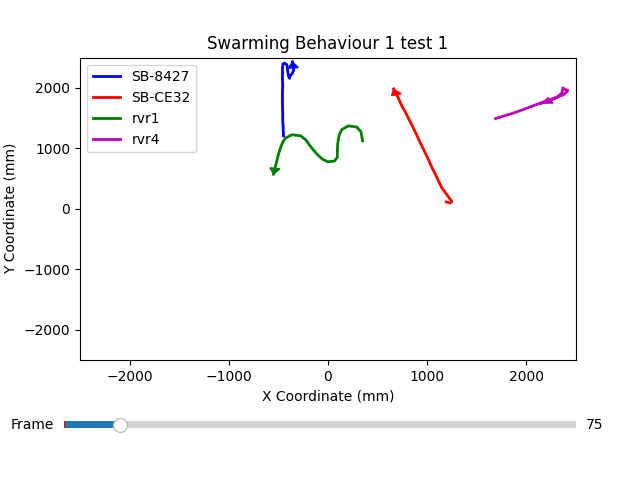
\includegraphics[width=0.4\textwidth]{appendix/Swarming Behaviour 1 test 1 plot.png}
    \caption{Location Plot for Swarming Behaviour 1 Test 1}
    \label{fig:swarming_behaviour_1_test_1}
\end{figure}

\begin{figure}[htbp]
    \centering
    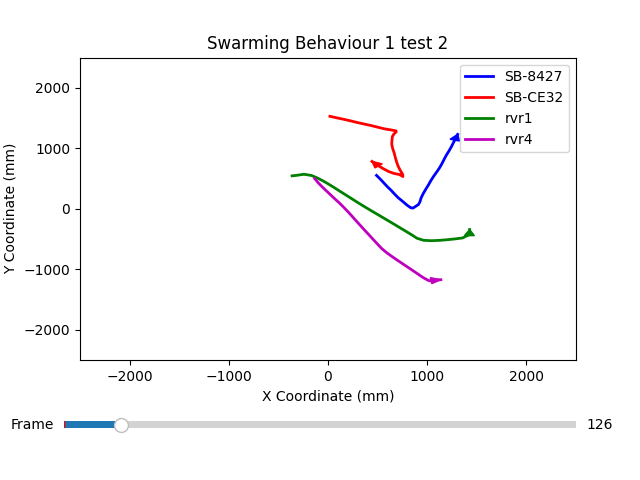
\includegraphics[width=0.4\textwidth]{appendix/Swarming Behaviour 1 test 2 plot.png}
    \caption{Location Plot for Swarming Behaviour 1 Test 2}
    \label{fig:swarming_behaviour_1_test_2}
\end{figure}

\begin{figure}[htbp]
    \centering
    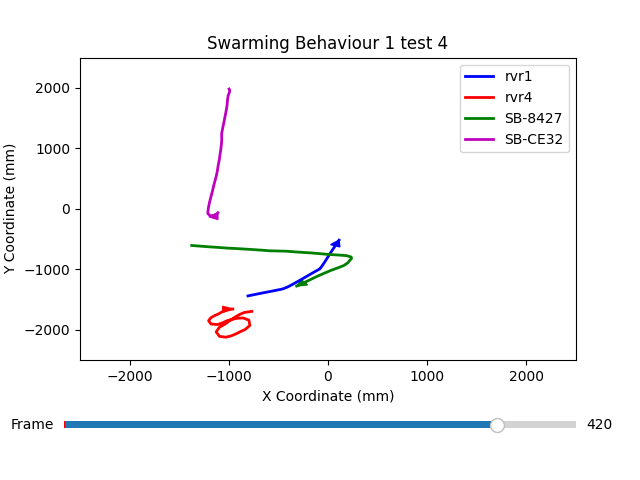
\includegraphics[width=0.4\textwidth]{appendix/Swarming Behaviour 1 test 4 plot.png}
    \caption{Location Plot for Swarming Behaviour 1 Test 4}
    \label{fig:swarming_behaviour_1_test_4}
\end{figure}

\begin{figure}[htbp]
    \centering
    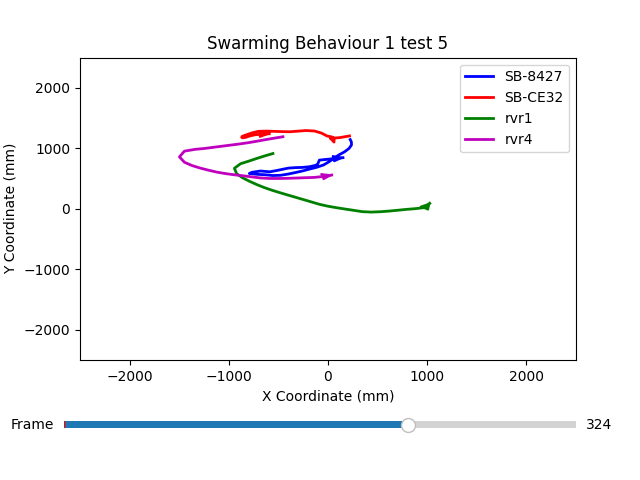
\includegraphics[width=0.4\textwidth]{appendix/Swarming Behaviour 1 test 5 plot.png}
    \caption{Location Plot for Swarming Behaviour 1 Test 5}
    \label{fig:swarming_behaviour_1_test_5}
\end{figure}

\begin{figure}[htbp]
    \centering
    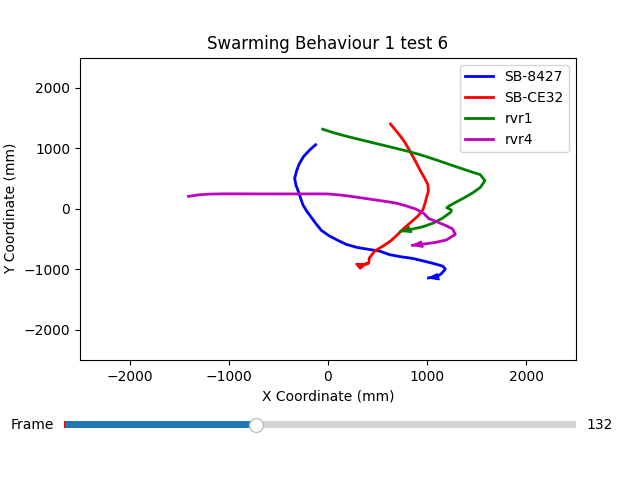
\includegraphics[width=0.4\textwidth]{appendix/Swarming Behaviour 1 test 6 plot.png}
    \caption{Location Plot for Swarming Behaviour 1 Test 6}
    \label{fig:swarming_behaviour_1_test_6}
\end{figure}

\begin{figure}[htbp]
    \centering
    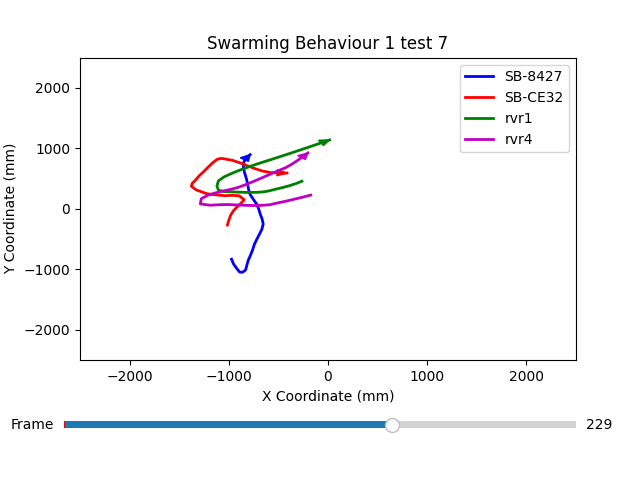
\includegraphics[width=0.4\textwidth]{appendix/Swarming Behaviour 1 test 7 plot.png}
    \caption{Location Plot for Swarming Behaviour 1 Test 7}
    \label{fig:swarming_behaviour_1_test_7}
\end{figure}

\begin{figure}[htbp]
    \centering
    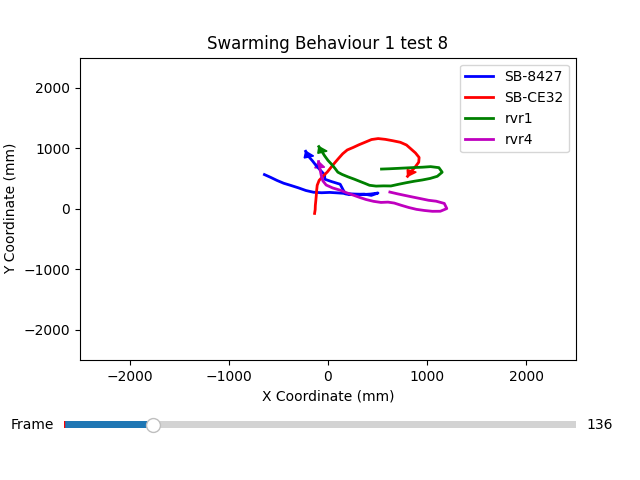
\includegraphics[width=0.4\textwidth]{appendix/Swarming Behaviour 1 test 8 plot.png}
    \caption{Location Plot for Swarming Behaviour 1 Test 8}
    \label{fig:swarming_behaviour_1_test_8}
\end{figure}

\begin{figure}[htbp]
    \centering
    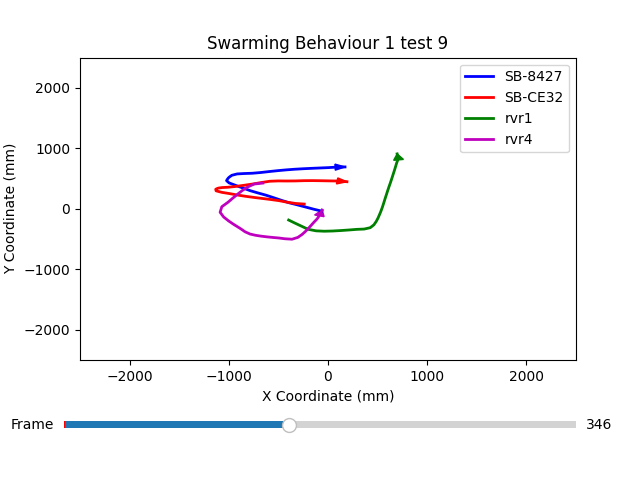
\includegraphics[width=0.4\textwidth]{appendix/Swarming Behaviour 1 test 9 plot.png}
    \caption{Location Plot for Swarming Behaviour 1 Test 9}
    \label{fig:swarming_behaviour_1_test_9}
\end{figure}

\begin{figure}[htbp]
    \centering
    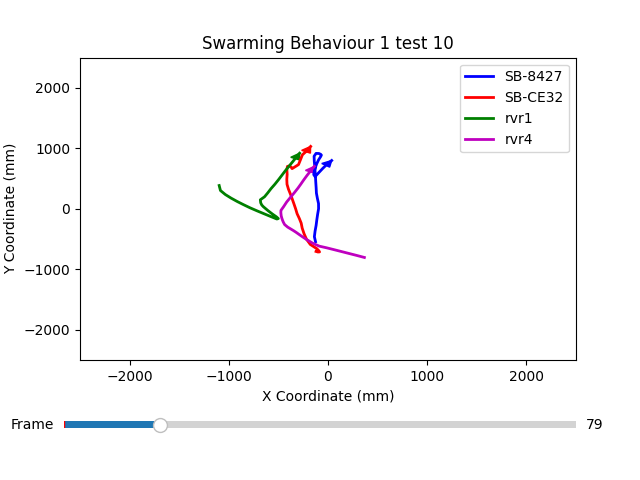
\includegraphics[width=0.4\textwidth]{appendix/Swarming Behaviour 1 test 10 plot.png}
    \caption{Location Plot for Swarming Behaviour 1 Test 10}
    \label{fig:swarming_behaviour_1_test_10}
\end{figure}

\begin{figure}[htbp]
    \centering
    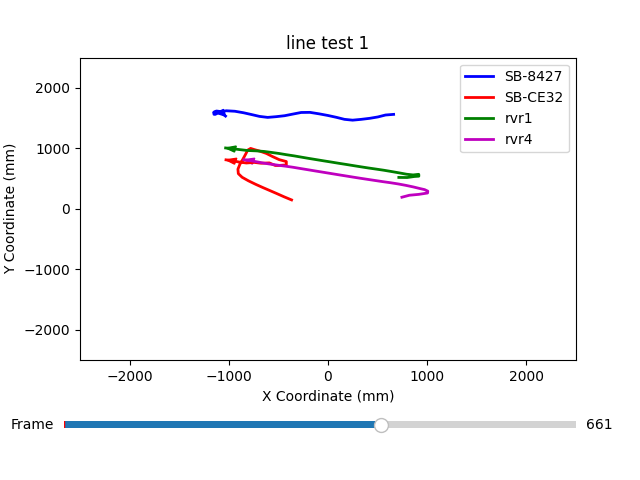
\includegraphics[width=0.4\textwidth]{appendix/line test 1 plot.png}
    \caption{Location Plot for Line Test 1}
    \label{fig:line_test_1}
\end{figure}


\end{document}
